\documentclass[12pt, a4paper]{article}
\usepackage[english]{babel}
\usepackage[utf8]{inputenc}
\usepackage{setspace}
\usepackage[bookmarksopen,colorlinks,linkcolor=black,urlcolor=Blue,citecolor=black]{hyperref}
\usepackage{multirow}
\usepackage{enumerate}
\usepackage{graphicx}
\usepackage{array}
\usepackage{caption}
\usepackage{float,lscape}
\usepackage{longtable}
\usepackage[margin=2.54cm, include foot]{geometry}
\usepackage{enumitem}
\usepackage{wrapfig}
\usepackage{threeparttable}
\usepackage{multicol}
\usepackage{dcolumn}
\usepackage{geometry}
\usepackage{makecell}
\usepackage{amsmath}
\usepackage[nameinlink]{cleveref}
\usepackage{appendix}
\usepackage{mathtools}
\usepackage{booktabs}
\usepackage{subcaption}
\usepackage[T1]{fontenc}
\usepackage{rotating}
\usepackage[natbibapa]{apacite}
\usepackage[usenames,dvipsnames]{color}
\usepackage{afterpage}
\usepackage{bbm}
\usepackage{pdflscape}
\hypersetup{
	colorlinks,
	citecolor=Blue,
	linkcolor=Blue,
	}
\usepackage{titling}

\begin{document}
\renewcommand{\BOthers}[1]{et al.\hbox{}}
\newcommand\fnote[1]{\captionsetup{font=footnotesize}\caption*{#1}}
\thanksmarkseries{alph}
\input{Tables/numbers.txt}

%\vspace{-2.35cm}
\title{\Large \textbf{Life in the Health Lane: The Professional Trajectories of Healthcare Workers in Colombia} \vspace{-0.1cm}}
\author{Grey Ceballos\thanks{\textit{Universidad EAFIT}, Carrera 49 N° 7 Sur-50, Medellin, 05001, Colombia (\href{mailto:gyceballog@eafit.edu.co}{gyceballog@eafit.edu.co}).} \and Pablo Uribe\thanks{World Bank, 1818 H Street NW, Washington DC, 20433, USA (\href{mailto:puribebotero@worldbank.org}{puribebotero@worldbank.org}).} \and Daniel Márquez\thanks{\textit{Universidad EAFIT}, Carrera 49 N° 7 Sur-50, Medellin, 05001, Colombia (\href{mailto:dmarquezm@eafit.edu.co}{dmarquezm@eafit.edu.co}).} \and Christian Posso\thanks{\textbf{Corresponding author:} \textit{Banco de la República}, Calle 50 \# 50-21, Medellin, 05001, Colombia (\href{mailto:cpossosu@banrep.gov.co}{cpossosu@banrep.gov.co}). The findings, interpretations, and conclusions expressed in this paper do not necessarily reflect the views of \textit{Banco de la República} or its Board of Directors. The authors’ names are listed in random order. Declarations of interest: none. This research did not receive any specific grant from funding agencies in the public, commercial, or not-for-profit sectors. We thank Juan David Rengifo for his excellent research assistance. We thank Andrea Otero and seminar participants at Universidad EAFIT, Universidad de Antioquia, and Banco de la República de Colombia for their insightful comments.}}
\maketitle

\vspace{-0.5cm}

% \begin{center}
%     \Large \textcolor{red}{This is a preliminary draft of an ongoing project. Please do not share}
% \end{center}

%%%%%%%%%%%%%%%%%%%%%%%%%%%%%%%%%%%%%%%%%%%%%%%%%%%%
\begin{abstract}
    
This paper studies the initial trajectories of healthcare professionals in the Colombian labor market, graduate school, and health. Leveraging comprehensive longitudinal administrative records for the universe of physicians, nurses, dentists, and bacteriologists, we employ a staggered event study framework to examine their early-life trajectories before and after their bachelor studies between 2008 and 2022. Key findings reveal substantial returns in the labor market for health professionals, with gender wage gaps and disparities in postgraduate enrollment. Furthermore, our analysis sheds light on the limited evidence concerning bad health trajectories, uncovering increased probabilities of emergency room visits and hospitalizations after graduation, particularly for nurses. Finally, our findings reveal that the prevalence of mental disorders increases for dentists and nurses after graduation, whereas for physicians, it decreases.

\end{abstract}


\textit{\textbf{Keywords:}} Healthcare Workforce, Healthcare workers’ working conditions, and mental health, Health postgraduate enrollment


\textit{\textbf{JEL Classification:}} I19, I26, J24, J31, J44

\vspace{.5cm}

\newpage
%%%%%%%%%%%%%%%%%%%%%%%%%%%%%%%%%%%%%%%%%%%%%%%%%%%%
\section{Introduction}

This paper studies the initial trajectories of healthcare professionals in the labor market, graduate school, and health. These professionals have been studied in different settings, emphasizing physicians and nurses \citep{okeke2023doctor,Posso2024births,chen2021team,doyle2010returns,antonazzo2003labour,Finkelstein2023,andreassen2017nurses,dunn2014physicians}. Nonetheless, less is known about the initial stages of their professional life and the heterogeneities within and between professionals. 

This paper closes the gap in the literature by showing how early healthcare graduates behave in terms of their labor supply decisions, earnings, and human capital accumulation at the postgraduate level. It also measures how the likelihood of a bad health shock and the risk of mental health disorders change after graduation. We study these trajectories by systematically analyzing detailed longitudinal administrative records of the universe of physicians, nurses, dentists, and bacteriologists, who obtained their degrees between 2011 and 2017. We focus on these four occupations since they are the only ones required to participate in a compulsory social service upon graduation and are considered of national interest in Colombia (see \autoref{sec:context} for more details).\footnote{In the Compulsory Social Service, the new graduates must provide professional services in urban and rural areas with limited access to health services. The service is provided once, right after obtaining the professional degree, and is a requirement for obtaining the professional license \citep{Minsalud2007}} 

Our data quality enables us to track these professionals before and after graduation from college across the labor market, education, and health dimensions. We exploit the graduation date of individuals in an event study framework to follow their life trajectories relative to the moment of their graduation. To achieve this, we use the \citet{callaway2021difference} estimator to control for key individual characteristics, temporal factors surrounding the graduation date, and to account for all group-time specific effects.\footnote{We estimate the universal event study aggregation from \citet{callaway2021difference}'s methodology, which allows us to interpret point estimates as the relative effect in a given year with respect to the pre-graduation period.} Considering the profound ``feminization'' of health personnel in Colombia \citep{Minsalud2018}\footnote{This is a common characteristic in many healthcare systems. According to the \citet{WHO2019}, women account for 70\% of the health and social care workforce and deliver care to around 5 billion people.}, we present our results and analyses differentiated between majors, and between gender for each profession, which allows us to reveal potential gender gaps.\footnote{\cite{Posso2024gender} use experimental variation to study the gender gaps in the physician market. Sex and gender will be used interchangeably across the paper.}

We build a unique panel that links three Colombian administrative records: the National Registry of Healthcare Talent, known as ReTHUS \citep{baserethus}, which provides information on the graduation date from any health program; the Integrated Contribution Payment, known as PILA \citep{basepila}, which contains mandatory contributions to health and pension for all employees in the country; and the Individual National Health Services Registry, known as RIPS \citep{baserips}.

Our empirical analysis delves into the dynamics of post-graduation trajectories, considering individual characteristics, temporally aggregated shocks surrounding the graduation date, and specific cohorts of professionals. Our observations underscore the heterogeneity of trajectories across different types of majors and gender. Our reduced form exercises are implicitly related to the dynamic discrete choice models in the returns to education literature.\footnote{Our research is also related with the large literature in economics that focuses on estimating the causal relationship between college education and earnings \citep{Patrinos2018}.} First, this literature shows that the choice of attending college and programs is determined by the forward-looking behavior of individuals, which depends on ex-ante characteristics associated with the varying nature of their ability and skills \citep{heckman2018returns,ge2013estimating}. Second, it also relates to the specialization through their choice of college major and their heterogeneous returns on the labor market \citep{Arcidiacono2020, Altonji2016}. Although we do not provide estimates of primitive parameters of the major and labor market decision-making, we provide well-estimated effects of the initial professional trajectories, not only in the labor market but in postgraduate education and health markets. 

We highlight four key findings. First, health professionals exhibit relatively high returns in terms of their employment prospects upon completing their bachelor studies. Notably, physicians emerge as the primary beneficiaries in the labor market, a trend attributed partly to their intensive work commitments. 

Second, there are important labor market gender gaps. While men and women in medicine and bacteriology exhibit similar monthly workdays, a notable disparity emerges among nurses and dentists, with women consistently working more days per month. Within the first year of entering the labor market, a noticeable gender wage gap emerges in medicine and nursing, with males consistently earning more than females. This gap widened significantly during the initial semesters but stabilized towards the end of our analysis period. Notably, the gender wage disparity within occupations, as observed in medicine and nursing, cannot be fully attributed to childbirth \citep{bertrand2010dynamics, goldin2014grand, goldin2011cost}\footnote{We also show that the trajectory on the probability of being pregnant is very similar between professions, there are no systematic differences.} or men having multiple jobs. 

Third, we dig into the enrollment trajectories in health postgraduate programs among physicians and dentists.\footnote{It's worth noting that data for other professionals in this outcome are unavailable.} Across many countries, pursuing postgraduate degrees in health-related fields is important for these professions due to the high demand for their services and the limited availability of workers in these areas. Our analysis unveils a comparable slow-increasing enrollment pattern for physicians and dentists during the initial two years after graduation. Subsequently, while the enrollment rate stabilizes for dentists, it continues to ascend for physicians, reaching its peak four and a half years after graduation. By the conclusion of our analysis period, approximately 14 percent of physicians are enrolled in health postgraduate programs, contrasting with just over seven percent of dentists.

Similar to wages, notable gender gaps persist in postgraduate education enrollment. From the first year after graduation, male physicians are more likely to enroll in health postgraduate programs than their female counterparts. Three years post-graduation, the gender disparity in postgraduate enrollment stabilizes at approximately one percentage point, which represents between 11.6\% and 26.7\% of the increase in male enrollment. This result is related to what is referred to as the “glass ceiling”, or the fact that women are underrepresented in top positions in society \citep{goldin2014grand}. 

Fourth, there is limited evidence on the initial health trajectories of healthcare professionals. We focus on analyzing trajectories of bad health events after the beginning of their professional career. There is evidence that the nature of the work carried out by healthcare professionals is associated with higher health risks \citep{mohanty2019health,kobo2023causes}. 
Notably, due to constant exposure to various occupational hazards such as frequent contact with patients, body fluids, bio-mechanical risks, and activities involving chemical handling, diagnostic imaging, radio-pharmaceuticals, and nuclear medicine, health professionals are often categorized as high-risk occupations in Colombia \citep{Ministeriodetrabajoyseguridadsocial}. Using our claim health data (RIPS), we measure bad health events as either an emergency room (ER) visit or a hospitalization \citep{hansagi2001frequent}. Such events are associated with a service that indicates poor health, where a person's life is at risk and requires immediate attention (ER visits) or prolonged direct care (hospitalization). 

On average, nurses, physicians, and bacteriologists exhibit the largest surge in the probability of emergency room (ER) visits after attaining their degrees. Notably, nurses show a remarkable increase of approximately 52 percent in the probability of ER visits within one year from graduation compared to the pre-graduation period. This trend persists even after four years. Conversely, no significant changes are observed for dentists after graduation. While occasional periods exhibit higher effects for women in medicine and bacteriology, there are no persistent gender gaps observed in this context. Furthermore, we investigate whether the heightened probability for women is driven by pregnancy by estimating regressions on the probability of ER visits unrelated to pregnancy. Remarkably, the results remain virtually unchanged, highlighting that pregnancy is not the primary driver behind the increased access to the ER for women. 

Similarly, all professionals are more likely to be hospitalized one year after graduation, with this probability escalating over time, particularly for nurses and bacteriologists. Our results suggest that nursing may entail harsher job conditions than other professions. Moreover, the effects are more pronounced for women across professions. However, it's worth noting that a portion of this gender gap is attributed to childbirth, which often requires hospitalization. By discounting the effect of pregnancy from women's estimates, we posit that while overall hospitalizations pose a significant health risk among all professionals, gender disparities within occupations are primarily evident for only nurses and dentists.

Finally, we examine the professional trajectories of mental health. Ample evidence exists regarding the prevalence of mental illnesses and burnout among healthcare professionals, with studies documenting their detrimental effects on the well-being of this population \citep{lai2020factors,young2021health, gold2013details,johnson2018mental,west2020resilience}. The demanding and stressful nature of the healthcare occupation predisposes workers to an elevated risk of developing negative mental states such as depression, anxiety, and stress \citep{ghazwin2016association,huang2018risks,maharaj2019prevalence}. Importantly, these health problems constitute an additional cost borne by healthcare workers that often goes unrecognized. 

Given the nature of our health data, we focus on measuring prevalence rather than incidence. Our health claims data measures medical diagnoses of mental illnesses rather than episodes. Once a diagnosis is determined, most mental illnesses are long-term conditions. Our results indicate that dentists and nurses increase their probability of having a mental condition by just over one percentage point by the fourth year after graduation, representing a relative effect of 35\% and 26\%, respectively. On the other hand, physicians decrease their probability by almost 1.5 percentage points after four years, consistent with a 37\% reduction. One possible explanation for this result is the demanding nature of undergraduate programs in medicine. Although their work can be as stressful as their studies, physicians face promising job prospects once they graduate. An alternative reasonable explanation is that physicians are avoiding revealing their mental conditions as a way to steer clear of negative prejudices. These findings underscore the considerable heterogeneity in health risk and mental health among healthcare professionals, emphasizing the need for targeted interventions to mitigate occupational health hazards.

The rest of the paper is organized as follows. Details on the specific context of healthcare workers within the Colombian health system are provided in \autoref{sec:context}. Then, \autoref{sec:data} describes the main data sources and shows descriptive statistics for our sample. Additionally, \autoref{sec:empirical} details the empirical strategy used to estimate our monetary and non-monetary incentives, and \autoref{sec:results} shows the results of such estimations. Finally, \autoref{sec:conclusion} concludes.


%%%%%%%%%%%%%%%%%%%%%%%%%%%%%%%%%%%%%%%%%%%%%%%%%%%%
\section{Setting} \label{sec:context}

In this section, we describe our setting. We start by describing Colombia's main requirements for being a health professional and the labor regulations that affect them. Then, we provide the main details about the postgraduate health training system. Finally, we briefly describe the Colombian health insurance system where health professionals work but are also patients.

\subsection{Healthcare workers}

There are three main requirements for professionals who wish to practice a healthcare profession in Colombia. First, they should have a degree granted by a legally recognized higher education institution.\footnote{The Ministry of Education must present the respective validation if a foreigner obtains the degree.} Recent figures from the National Registry of Healthcare Talent (ReTHUS, by its Spanish acronym)\footnote{\textit{Registro Único Nacional del Talento Humano en Salud.}} show the number of new professionals in bacteriology, nursing, medicine, and dentistry has grown an average of 11,154 per year between 2010 and 2020. By 2021 there were 157,096 physicians, 77,997 nurses, 28,128 bacteriologists, and 63,965 dentists.\footnote{Colombia's population in 2022 was 51,874,024.} This is consistent with the number of higher education institutions offering a health-related program, which has been rapidly growing. For instance, in 2001, there were 87 bacteriology, nursing, medicine, and dentistry programs; nowadays, there are 238 \citep{SPADIES}. This has led to significant heterogeneities in the quality of healthcare professionals,\footnote{\citet{Posso2024births} report this heterogeneity for the case of medicine.} as many of them obtain their degrees in non-accredited or newly-formed institutions.

Second, for the particular case of professionals in bacteriology, nursing, medicine, and dentistry, they must prove compliance with the Compulsory Social Service (SSO, by its acronym in Spanish),\footnote{\textit{Servicio Social Obligatorio}.} which is accessed through a national contest. In this compulsory service, new graduates must provide professional services in urban and rural areas with limited access to health services for one year before practicing as professionals. It was created by Law 50 of 1981, later modified by Law 1164 of 2007, and ultimately regulated in Resolution 774 of 2022. The service is provided once, right after obtaining the professional health degree, and is a requirement to obtain the professional license \citep{ley1164}. 

The number of slots for social services is limited. As of December 31, 2022, the annual offer included 5,409 Compulsory Social Service slots distributed throughout the national territory. There were a more significant number of positions in medicine (73.1\%), followed by nursing (13.0\%), dentistry (8.2\%), and bacteriology (5.6\%) \citep{SISPRO}. Therefore, all graduates must appear for the call. Professionals who do not obtain one of the slots for the SSO will be exonerated and can immediately obtain the professional license.\footnote{Currently, the Ministry of Health and Social Protection makes the call four times a year. The professional selected to occupy an SSO position who does not occupy it or renounces it before the term is disqualified for nine months from appearing for a new call. Professionals assigned to social service positions may receive salary and non-salary incentives such as payment for transportation, accommodation, food, and others \citep{Minsaludyprotecciónsocial}.}

Third, they must enroll in ReTHUS, which can only happen once individuals have met the two former requirements. Since Law 1164 of 2007, every individual who intends to exercise a healthcare profession or occupation in Colombia, whether at an auxiliary, technical, technologist, or professional level, must register in ReTHUS. After successful registration, the professional will be issued the Unique National Identification of Human Talent in Health card. This procedure generates the administrative act (Resolution), which authorizes people to exercise their profession or occupation throughout the national territory. ReTHUS contains detailed information on the individuals who have met the requirements to practice in the health sector. 

Once licensed, health professionals in Colombia are governed by the same labor regulations as other citizens. According to Decree 1607 of 2002, all workers in Colombia with a legally constituted contract must be affiliated with the General Occupational Risk System, a subsystem of the General System of Social Security (SGSS, by its Spanish acronym).\footnote{Decree 1607 of 2002 was repealed by Decree 768 of 2022; however, given that our data corresponds mainly to the period before 2022, we will use Decree 1607.} The company's economic activity determines the risk level according to the International Standard Industrial Classification. The risk classification varies between 1 and 5, with 5 being the highest risk. For most healthcare workers, the risk level is 3, given the constant interaction with humans, body fluids, and associated biomechanical risks. Some professionals who work in medical and dental practice companies without hospitalization or emergencies could report risk level 1, and other professionals report risk level 5 when their work activity is related to handling chemicals or diagnostic imaging, radio-pharmaceuticals, or nuclear medicine \citep{Ministeriodetrabajoyseguridadsocial}.


\subsection{Postgraduate degrees in health }

Once health professionals have graduated and meet the basic requirements to practice the profession (including the SSO), they can aspire to postgraduate training, which can be clinical and surgical specialties or research-type degrees such as master's and doctorate. Postgraduate training is in charge of higher education institutions, and the number of slots for specialties in medicine is particularly limited. According to \cite{trejos2022consideraciones}, one out of every four medical professionals enters graduate school in medicine.\footnote{In the U.S., one out of every two physicians has a specialty \citep{Statista}.} Universities have autonomy in the number of places they offer and in the admission process, which may include one or more of the following requirements: knowledge tests, English proficiency, personal interviews, and research experience.

The training for medical and dental specialties lasts two to five years, and sub-specialty training lasts one to two more years. The full-time student carries out the training exclusively in person. In a specialty such as internal medicine, students must pay an amount that can vary between 3,500 to 7,000 USD per academic period (semester or year), with few exceptions \citep{HernándezandSierra}. However, these costs are likely to be recovered quite fast. For instance, physicians with a clinical specialty had an average monthly salary of approximately 3,926 USD in 2021, while surgical specialists earned 4,368 USD.\footnote{Real salaries are calculated using 2018 as the base period and the average 2021 exchange rate of 3,744 COP per USD. According to OECD, the purchasing power parity (PPP) Colombian pesos/US dollars in 2021 was 1,317.} These salaries are equivalent to 16 and 18 times the monthly minimum wage in Colombia, respectively. In the case of dentists, those with postgraduate degrees had an average monthly salary of 1,134 USD in 2021, equivalent to 4.6 times the monthly minimum wage. Their income is likely to be larger than this, but as will be shown in this paper, there might be considerable under-reporting of wages in this profession.

When professionals enroll in a postgraduate degree in health, academic internships in health institutions are required. They must contribute to the General Occupational Risk System throughout their training and register under code 21 as postgraduate health students according to Decree 780 of 2016. Physicians and dentists frequently pursue these postgraduate programs to attain specialty or sub-specialty in their respective fields. However, postgraduate training in nursing and bacteriology differs from that in medicine and dentistry, typically spanning one to two years, and institutions are not required to register them under code 21. Exclusive dedication from the student is not mandatory. Therefore, they can maintain professional ties with a company while completing their clinical or research-based postgraduate studies.


\subsection{The Colombian healthcare system}

Colombia has a social security system that encompasses healthcare, pension, and professional risk management for the formally employed. Within this system is a subsystem called the General System of Social Security in Health (SGSSS, by its Spanish acronym).\footnote{\textit{Sistema General de Seguridad Social en Salud.}} It relies on the principles of universality and equity to ensure access to services for the entire population. Health insurance coverage has increased substantially over the last decades, reaching 99.6\% in 2022 \citep{Minsalud2022}. This guarantees coverage of a wide range of services, including visits to outpatient general practitioners and specialists, inpatient care, and prescription drugs with little to no co-payments. The system relies on three main actors: government, health insurers (EAPB, by its Spanish acronym),\footnote{\textit{Entidades Administradoras de Planes de Beneficio.}} and healthcare providers (IPS in Spanish).\footnote{\textit{Instituciones Prestadoras de Salud}.} Additionally, the SGSSS is structured into special, contributory, and subsidized regimes, with the last two being the most prominent.

Residents in Colombia are necessarily affiliated with an EAPB of either the contributory or subsidized regimes, depending on their economic capacity. The contributory regime encompasses formal employees, retirees, and self-employed individuals who earn at least the minimum wage. It is funded through the contributions of its members, with a portion of these funds allocated to support the subsidized system as well. Conversely, the subsidized regime is designed to provide healthcare services to the most economically disadvantaged population in the country. This group, which lacks the financial means to cover healthcare expenses, receives government subsidies to ensure access to essential medical care. Interestingly, the health benefits plan is the same across regimes.

To get access to health services, individuals in the contributory regime must pay a moderator fee, which is a negligible monetary contribution whose purpose is to regulate the use of health services and encourage their proper use. Its value varies according to the monthly income of the dependent or self-employed worker. In addition, for each health service provided, individuals must make a co-payment, which corresponds to a share of the total value of the service provided and is intended to help finance the system. Co-payments depend on the regime and the individual's monthly income and are very low compared to the cost of the health service \citep{Aseguramiento}.

People who are part of the contributory regime must make monthly contributions as a function of their wages. These contributions are split between the employer and the employee in the case of dependent workers. On the other hand, self-employed workers must cover the entirety of their required contribution but only using 40\% of their wage as the base for calculation \citep{Aseguramiento}.\footnote{The required contributions are of 12.5\% of the base to health, 16\% of the base to pension funds, and a varying rate to risk managers between 0.522\% and 6.98\% depending on the occupational risk of the individual. For dependent workers, 75\% of the contribution is handled by the employer.} However, this contribution is self-reported for these individuals, and the only requirement is that it should at least be equal to the monthly minimum wage, even if 40\% of their income falls below it.\footnote{This may lead to many self-employed under-reporting their incomes.} All of these contributions are recorded in the \textit{Planilla Integrada de Liquidación de Aportes} (PILA), a system created by Resolution 1303 of 2005 of the former Ministry of Social Protection. Through an online form, employers' and employees' contributions to social security are integrated to avoid having to separately contribute to a pension, health, professional risks, and all other legally required sub-accounts.


\subsection{Healthcare services}

The general practitioner is the gateway to the health system. People with any health affliction must initially consult the general practitioner, who determines the probable diagnosis and procedures to follow. In that sense, they request complementary diagnostic aids, supply medications, and analyze the need to continue the process with a specialist or another health professional. Additional procedures and referrals to other specialties require authorization from the EAPB, who makes the payments for the provided service. Any individual can go directly to a specialist without going through the general practitioner by setting a ``private'' appointment. However, the diagnostic and medical aid derived from this type of consultation must be paid for in its entirety by the person.

Regardless of the type of physician that provides the service to an individual or whether it is a private appointment, information is centralized in the Individual National Health Services Registry (RIPS, by its acronym in Spanish).\footnote{\textit{Registros Individuales de Prestación de Servicios de Salud.}} These records are the set of minimum and basic data that the General System of Social Security in Health requires for the management, regulation, and control processes for all health service provider institutions (IPS) and other actors in the system. Thus, the registration of provided healthcare services information is mandatory for all providers, in accordance with Resolution 3374 of 2000 \citep{RIPS}. This implies that any service a user demands must be recorded in RIPS, including the diagnostic codes associated with the user's reason for the visit. Diagnoses are coded following the International Classification of Diseases ICD-10 \citep{RIPS}.


%%%%%%%%%%%%%%%%%%%%%%%%%%%%%%%%%%%%%%%%%%%%%%%%%%%%
\section{Data} \label{sec:data}

We merge comprehensive national administrative records from all physicians, nurses, dentists, and bacteriologists active between 2008 and 2022. In this section, we provide details on the three main data sources. In \autoref{sec:data_appendix}, further details are provided on the process we follow to merge the data. For the main empirical exercise, we focus on professionals who graduated between 2012 and 2017.\footnote{We choose this window to be able to follow individuals two years before obtaining their degree and up to five years after that.} 


\subsection{ReTHUS: National Registry of Healthcare Talent}


 ReTHUS contains information on individuals who have met the requirements to exercise their profession within the healthcare system in Colombia. It includes specific details like the individual's gender, type of bachelor's degree obtained and graduation dates, whether the individual obtained a postgraduate degree in health and graduation dates, and when they obtained the professional license. We identify \samplerethus\ individuals who graduated from the four professions that require the SSO (bacteriology, medicine, nursing, and dentistry) between 2011 and 2017.\footnote{We only focus on individuals who do not have multiple undergraduate degrees (see \autoref{sec:data_appendix} for details).} This represents around 59\% of the healthcare professionals in the country who graduated in that same time span, and it is our main dataset.

\subsection{RIPS: Individual National Health Services Registry}

RIPS is the Colombian national administrative record of all medical consultations, health procedures, emergency room visits, and hospitalizations. It contains individuals' identifications, age, gender, and the diagnosis code corresponding to the pathology originating the signs and symptoms for which the user needed to visit the healthcare provider. We use yearly information from 2009 to 2022 across all health services and match these registries to ReTHUS to build a longitudinal dataset that tracks the professionals' health outcomes up to five years after graduation.\footnote{We decide to use yearly data to capture low-incidence diseases.} With these data, we can identify whether an individual suffered from a particular disease in a given year, the number of services demanded, and even the types of physicians consulted.


\subsection{PILA: Integrated Contribution Payment from Colombia’s Ministry of Health and Social Protection}


PILA offers a thorough record of monthly contributions made by individuals towards healthcare, pension funds, and occupational risk insurance. It contains individuals' identifications, date of birth, gender, and extensive details regarding earnings, the number of days worked, and employer characteristics for all formally employed individuals in Colombia. We collapse the data at the semester level to ensure the tractability of the information.\footnote{The conclusions remain the same if we use monthly or annual data.} We use information from PILA between 2008 and 2022 and match these registries to ReTHUS to build a longitudinal dataset that tracks the professionals' involvement in the formal labor market up to five years after graduation. We mainly focus on the median monthly real income, the number of days worked per month, whether individuals had multiple jobs and their contract type. As explained in \autoref{sec:data_appendix}, our definition of income includes the sum of all salaries received in the month in cases where individuals have multiple jobs. Additionally, PILA contains information on whether the individual is enrolled in a postgraduate health-related degree. This is possible since all higher education institutions in Colombia are required by law to affiliate their postgraduate students to social security \citep{Minsalud}.

\subsection{Summary statistics}

The summary statistics for our data are shown in \autoref{tab:rethus_summary}. It shows that 49\% of our sample are physicians, with the majority being females, while only 6\% are bacteriologists. Overall, 70\% of healthcare workers are female, most of whom are physicians or nurses.

\begin{table}[H]
  \centering
  \caption{Main sample statistics}
  \resizebox{\textwidth}{!}{
  \begin{threeparttable}
    \begin{tabular}{cccccc}
    \toprule
    \multicolumn{1}{r}{} & All professions & Bacteriologists & Nurses & Physicians & Dentists \\
    \midrule
    \multicolumn{1}{l}{Whole sample} & 77,900 & 4,849 & 22,138 & 38,130 & 12,783 \\
    \multicolumn{1}{r}{} & (100\%) & (6.22\%) & (28.42\%) & (48.95\%) & (16.41\%) \\ \addlinespace
    \multicolumn{1}{l}{Males} & 23,275 & 761   & 2,773 & 16,243 & 3,498 \\
    \multicolumn{1}{r}{} & (29.88\%) & (0.98\%) & (3.56\%) & (20.85\%) & (4.49\%) \\ \addlinespace
    \multicolumn{1}{l}{Females} & 54,625 & 4,088 & 19,365 & 21,887 & 9,285 \\
    \multicolumn{1}{r}{} & (70.12\%) & (5.25\%) & (24.86\%) & (28.1\%) & (11.92\%) \\
    \bottomrule
    \end{tabular}%
  \begin{tablenotes}[flushleft] \footnotesize
\item \textit{Notes:} The proportions of individuals from each profession and gender with respect to the total sample are shown in parentheses. 
\end{tablenotes}
\end{threeparttable}}
  \label{tab:rethus_summary}%
\end{table}%

Additionally, \autoref{tab:pila_rips_all} shows the summary statistics for the labor market (panel A) and health variables (panel B) for the whole sample before and after graduation. The average formal real monthly wage was \meanwage\ COP (equivalent to around 508 USD)\footnote{Using the average 2018 exchange rate of 2,956 COP per USD.}. %Almost everyone in our sample (\meandependent\%) worked as a salaried employee (dependent) at least once between 2008 and 2022, and \meansimuljobs\% had simultaneous jobs. 
Also, around \meanpostgrad\% were enrolled in a health-related postgraduate program. Regarding healthcare utilization, \meanurg\% went to the ER, and \meanhosp\% were hospitalized at least once between 2009 and 2022. But most shockingly, \meanmentaldiag\% received a diagnosis related to a mental illness during this period.

\begin{table}[H]
  \centering
  \caption{Labor and health market statistics (whole sample)}
  \resizebox{.8\textwidth}{!}{
  \begin{threeparttable}
    \begin{tabular}{p{20.5em}cccc}
    \toprule
    \multicolumn{1}{r}{} & Mean & SD & Min & Max \\
    \midrule
    \multicolumn{5}{l}{\textit{Panel A: PILA (2008-2022)}} \\
    Monthly days worked & 13.449 & 6.022 & 0     & 30 \\
    Formal real monthly wage & 1,502,145 & 1,186,183 & 0     & 23,879,382 \\
    Health-related postgrad. enrollment & 0.151 & 0.359 & 0     & 1 \\
    Simultaneous jobs & 0.800 & 0.400 & 0     & 1 \\
    Self-employed workers & 0.784 & 0.412 & 0     & 1 \\
    Dependent workers & 0.968 & 0.177 & 0     & 1 \\ \addlinespace
    \multicolumn{5}{l}{\textit{Panel B: RIPS (2009-2022)}} \\
    Accessed a health service & 0.972 & 0.166 & 0     & 1 \\
    Medical consultations & 0.956 & 0.205 & 0     & 1 \\
    Medical procedures & 0.926 & 0.261 & 0     & 1 \\
    ER visits & 0.554 & 0.497 & 0     & 1 \\
    Hospitalizations & 0.214 & 0.410 & 0     & 1 \\
    Received mental diagnosis & 0.152 & 0.359 & 0     & 1 \\
    \bottomrule
    \end{tabular}%
  \begin{tablenotes}[flushleft] \footnotesize
\item \textit{Notes:} Summary statistics are for the entire period of each panel. Wages are in Colombian Pesos (COP). Individuals will take a value of one in all Panel B variables and Health-related postgrad. enrollment if the condition was met at least one month in the analyzed period. See \autoref{sec:data_appendix} for details on each of the variables. 
\end{tablenotes}
\end{threeparttable}}
  \label{tab:pila_rips_all}%
\end{table}%

\autoref{tab:pila_rips_gender} separates the previous statistics by gender. Right away, there is a significant wage gap between males and females. While the average formal real monthly wage for men was \meanwageM\ COP, for women it was \meanwageF\ COP. %Although women seem to have worked more days per month, \meansimuljobsM\% of men had simultaneous jobs at least once between 2008 and 2022, while \meansimuljobsF\% of women did. 
On the other hand, women appear to be more concerned about their health, since \meanconsulF\% of them went to a medical consultation between 2009 and 2022, while only \meanconsulM\% of men did. However, more females went to the ER and were hospitalized, on average, than men. Moreover, \meanmentaldiagF\% of women received a mental diagnosis while only \meanmentaldiagM\% of men did.

\begin{table}[H]
  \centering
  \caption{Labor and health market statistics (whole sample)}
  \resizebox{\textwidth}{!}{
  \begin{threeparttable}
    \begin{tabular}{lcccccccc}
    \toprule
    & \multicolumn{4}{c}{Males}     & \multicolumn{4}{c}{Females} \\
    \cmidrule(l){2-5} \cmidrule(l){6-9}         
    & Mean  & SD    & Min   & Max   & Mean  & SD    & Min   & Max \\
    \midrule
    \multicolumn{9}{l}{\textit{Panel A: PILA (2008-2022)}} \\
    Monthly days worked & 13.273 & 6.050 & 0     & 30    & 13.524 & 6.009 & 0     & 30 \\
    Formal real monthly wage & 1,768,995 & 1,490,024 & 0     & 23,879,382 & 1,388,444 & 1,008,626 & 0     & 22,972,394 \\
    Health-related postgrad. enrollment & 0.214 & 0.410 & 0     & 1     & 0.125 & 0.331 & 0     & 1 \\
    Simultaneous jobs & 0.827 & 0.379 & 0     & 1     & 0.788 & 0.409 & 0     & 1 \\
    Self-employed workers & 0.818 & 0.386 & 0     & 1     & 0.769 & 0.421 & 0     & 1 \\
    Dependent workers & 0.966 & 0.182 & 0     & 1     & 0.968 & 0.175 & 0     & 1 \\ \addlinespace
    \multicolumn{9}{l}{\textit{Panel B: RIPS (2009-2022)}} \\
    Accessed a health service & 0.947 & 0.223 & 0     & 1     & 0.982 & 0.134 & 0     & 1 \\
    Medical consultations & 0.921 & 0.270 & 0     & 1     & 0.971 & 0.168 & 0     & 1 \\
    Medical procedures & 0.863 & 0.344 & 0     & 1     & 0.953 & 0.211 & 0     & 1 \\
    ER visits & 0.494 & 0.500 & 0     & 1     & 0.579 & 0.494 & 0     & 1 \\
    Hospitalizations & 0.132 & 0.338 & 0     & 1     & 0.250 & 0.433 & 0     & 1 \\
    Received mental diagnosis & 0.123 & 0.328 & 0     & 1     & 0.165 & 0.371 & 0     & 1 \\
    \bottomrule
    \end{tabular}%
  \begin{tablenotes}[flushleft] \footnotesize
\item \textit{Notes:} Summary statistics are for the entire period of each panel. Wages are in Colombian Pesos (COP). Individuals will take a value of one in dummy variables if the condition was met at least one month in the analyzed period. See \autoref{sec:data_appendix} for details on each of the variables. 
\end{tablenotes}
\end{threeparttable}}
  \label{tab:pila_rips_gender}%
\end{table}%

Finally, \autoref{fig:hist} shows the distribution of our sample's graduation dates. The number of graduates has increased over time, and the total sample is distributed proportionally across cohorts. The majority of graduates do so in the second semester every year. This follows the same pattern as high school graduation in the country.\footnote{Colombia has two calendars for secondary education: A and B. Calendar A includes all public schools and most private schools.}

\begin{figure}[H]
\caption{Distribution of graduation dates}\label{fig:hist}
\centering 
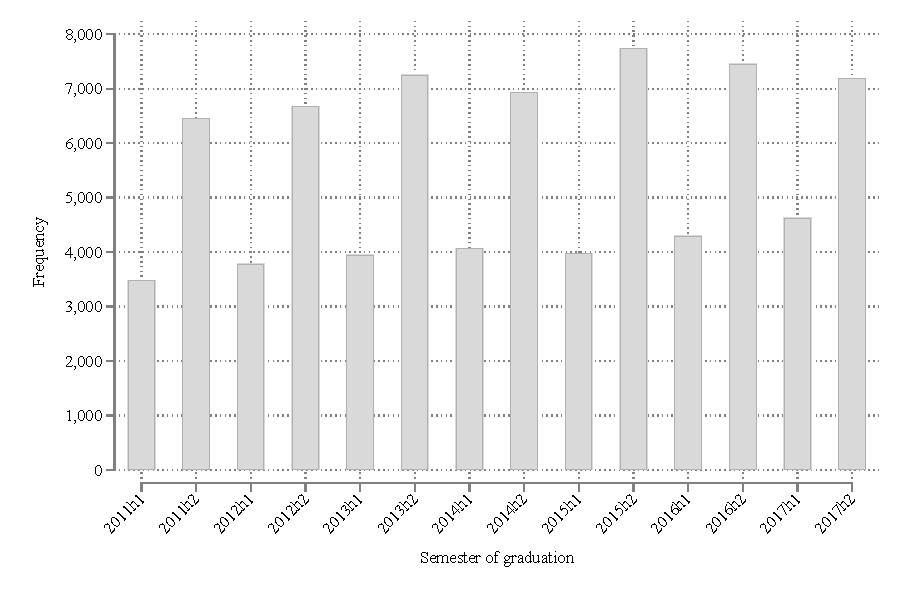
\includegraphics[width=\textwidth]{Figures/hist_graduates_sample_half.pdf}
\fnote{\textit{Notes:} Each bar shows the number of individuals from our sample who graduated in that given semester.}
\end{figure}


%%%%%%%%%%%%%%%%%%%%%%%%%%%%%%%%%%%%%%%%%%%%%%%%%%%%
\section{Empirical Strategy} \label{sec:empirical}

The main purpose of this section is to present a methodology that allows us to understand the impact of pivotal life events, such as the beginning of professional life, on individuals' labor, education, and health trajectories. We focus on dissecting the intricate dynamics of post-undergraduate-graduation trajectories from individual characteristics or specific cohorts of professionals. To do that, we build on a two-way fixed effects (TWFE) estimation to control for key individual characteristics and temporal factors surrounding the graduation date and ultimately use the \citet{callaway2021difference} (hereafter CS) estimator to account for all group-time specific effects.\footnote{In the main text, we focus on the CS estimator. TWFE is not included, yet it shows similar results.} Our baseline specification follows a TWFE regression as:

\begin{equation}
        Y_{it} = \alpha + \sum_{k=K}^{-2} \beta_k^{lead} D_{it}^{k} + \sum_{k=0}^{L} \beta_k^{lag} D_{it}^{k} + \gamma_t + \psi_i + \varepsilon_{it}
\end{equation}

\noindent where $Y_{it}$ is the labor, postgraduate, or health outcome of individual i at time t, and $\gamma_t$ and $\psi_i$ are time and individual fixed effects, respectively. Standard errors are clustered at the individual level. Additionally, $D_{it}$ is an indicator for individual \textit{i} being \textit{k} periods away from graduation at time \textit{t}, which can be expressed as:

\begin{equation} 
D_{it}^{k} = \mathbbm{1}(t - G_i = k) 
\end{equation}

Where $G_i$ indicates the period unit $i$ is first treated (group). The coefficients of interest are $\beta_k$, which capture the dynamic effects on our variables of interest relative to the pre-graduation period.\footnote{Labor market outcomes are semiannual while health outcomes are annual (see details in \autoref{sec:data_appendix}).} One key concern in the above setting is that different groups of individuals, for instance, specific cohorts of physicians or nurses, may experience different treatment effects. TWFE may not correctly account for these heterogeneities, creating bias in our estimates \citep{de2020two,roth2023whats}. With such heterogeneities, TWFE may include ``forbidden comparisons'' that could introduce negative weights to the regression and change the point estimate \citep{goodman2021difference}. This also implies that the pre-trends evaluation can be misleading since even under parallel trends, pre-treatment coefficients will not necessarily be zero \citep{sun2020csdid,roth2023whats}. 

To overcome these problems, we implement the \citet{callaway2021difference} estimation method, which avoids the negative weights problem by calculating all group-time-specific effects accounting for each group's size. One key characteristic of the CS estimator is that it does not require never-treated units, which is our case.\footnote{Designs with only eventually treated units are called stepped wedge designs.} In our setting, the CS estimator compares outcomes between periods t and the average over cohorts not yet treated in period t; i.e., those who will eventually graduate but have not yet graduated by the analyzed period.\footnote{This is particularly important since all individuals have already graduated, so there is no group of never-treated units. This is a particular advantage of CS over the \citet{sun2020csdid} method, which uses either the never-treated units or the last-to-be-treated units for comparisons instead of the not-yet treated \citep{roth2023whats}. On the other hand, the advantage of CS over imputation methods like \citet{borusyak2023revisiting} is that, in the latter, comparisons are made against the average of pre-treatment periods, imposing parallel trends across all of them, rather than only on post-treatment periods like CS. This may lead to a larger bias.} In \autoref{fig:hist}, we showed that we have fourteen biannual cohorts. CS will use the weighted average of the other 13 cohorts as a comparison group for the first-ever treated cohort. The same procedure is then repeated for the remaining cohorts.\footnote{When the outcome is measured annually we can count with seven cohorts.} 


%%%%%%%%%%%%%%%%%%%%%%%%%%%%%%%%%%%%%%%%%%%%%%%%%%%%
\section{Results} \label{sec:results}

This section presents the main results. We control all estimations for individuals' time-invariant characteristics and time-fixed effects while accounting for possible heterogeneities across cohorts using the \citet{callaway2021difference} estimator. All coefficients are relative to the immediate pre-graduation period, whose mean is shown in each figure's legend. This will allow us to interpret the results as conventional event studies. This section is organized as follows. In \autoref{sec:pila}, we show the professional trajectories of the four types of professionals: physicians, nurses, bacteriologists, and dentists. Then, \autoref{sec:rips} provides the results for their health-related trajectories.

Overall, we observe that the professional trajectories are heterogeneous by type of professional and gender. Physicians and nurses report working the most days per month after graduation and earning the highest formal real wages, although men appear to be earning higher salaries over time. In addition, physicians and nurses show a significant gender gap in wages starting one semester after graduation and increasing over time.

Moreover, these trajectories also depend on labor market institutions such as the types of contracts, number of jobs, and health graduate school. For instance, female dentists are more likely to be self-employed,\footnote{Self-employed workers in Colombia are responsible for reporting their salary.} working with health institutions for specific activities without a direct employment relationship or opening their private practices, where it is often difficult to verify profits. Both situations may then lead to under-reported wages.\footnote{Since a significant portion of dentists are self-employed, they could decide to allocate their practice income between salary and business profits, knowing that the latter does not have the same tax burdens.} On the other hand, physicians are, in general, more likely to have simultaneous jobs. While physicians and dentists are more likely to enroll in health postgraduate degrees over time, physicians have the edge over dentists in terms of salary.

Analyzing health trajectories, we have identified significant heterogeneity across professions and genders. Notably, nurses and physicians are more likely to go to the emergency room (ER) after graduation, and all four professionals face an increased probability of hospitalization. While there are no discernible gender-based differences within professions in ER visits, a notable one emerges for hospitalizations. This gap persists, particularly affecting women, with differences reaching one percentage point for physicians, two for dentists, and three for nurses. Excluding maternity-related hospitalizations reduces this gap by approximately one percentage point for the latter three professions. Regarding mental illnesses, nurses and dentists have a higher prevalence of mental diagnoses after graduation, while physicians show the opposite behavior.


\subsection{Labor market trajectories \label{sec:pila}}

We begin by looking at the professional labor trajectories in three main areas: labor supply, wages, and type (number) of jobs. As expected, all these outcomes are significantly affected after graduation, but there are important heterogeneities by type of profession and gender. These are mainly concentrated in wages and outcomes where gender gaps are more pronounced.

\subsubsection{Labor supply}

We focus on the intensive margins, measured in days worked per month.\footnote{In Colombia, health professionals have high levels of formality (extensive margin). In addition, formal workers in Colombia do not report the number of hours they work. Using household surveys from 2021 to 2023 (information is not available by profession in other years), we show the average number of hours reported between males and females within professions (see \autoref{fig:working_hours} in the appendix). Nurses work more hours than other professionals, while dentists work significantly fewer hours.} \autoref{fig:days} reports the trajectories for each of the four occupations in the number of days worked. On average, professionals work in jobs that demand one-tenth of a full-time schedule (measured as 30 days) before graduating with their bachelor's. This could be related to earlier experience or other work that allows students to cope with their education costs. Bacteriologists are the ones who work the highest number of days at that stage. However, most professionals work almost full-time after graduation. Physicians and nurses report working more days after graduation than other professionals, while the opposite happens for dentists. This might be explained by the more time-consuming nature of the medical degree, where physicians can only significantly increase their labor supply upon graduation and completion of the social service. As for dentists, the lower supply might be related to their higher propensity to report being self-employed and under-reporting salaries, which will be analyzed later.

\begin{figure}[H]
\caption{Monthly days worked}\label{fig:days}
\centering 
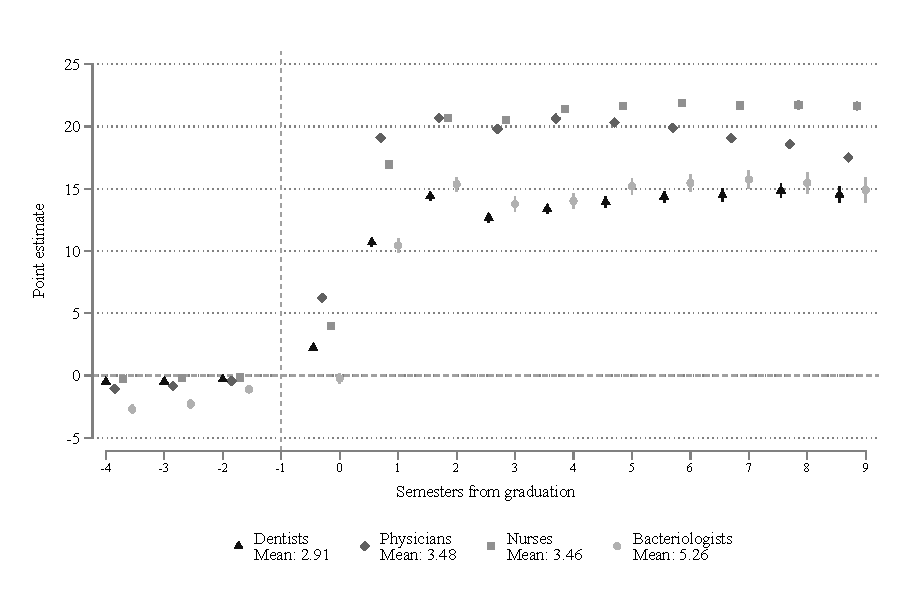
\includegraphics[width=\textwidth]{Figures/Callaway SantAnna/ES_sal_dias_cot_0_all.pdf}
\fnote{\textit{Notes:} Each point represents a coefficient from the \citet{callaway2021difference} estimation. The lines across the coefficients are confidence intervals at the 95\% level. Standard errors are clustered at the individual level. The outcome's mean at the baseline period (-1) for each profession is reported in the legend.}
\end{figure}

When separating the estimations by gender (see \autoref{fig:days_gender}), there are no significant differences between males and females for physicians and bacteriologists (see \autoref{fig:days_gap} in the appendix for the gap). On the other hand, female dentists and nurses seem to be working more days than their male counterparts.\footnote{ Using household surveys from 2021 to 2023, we show that there are no significant differences in the number of hours reported between males and females within professions (see \autoref{fig:working_hours} in the appendix.}

\begin{figure}[H]
\centering
\caption{Monthly days worked by gender}
\begin{subfigure}{.5\textwidth}
  \centering
  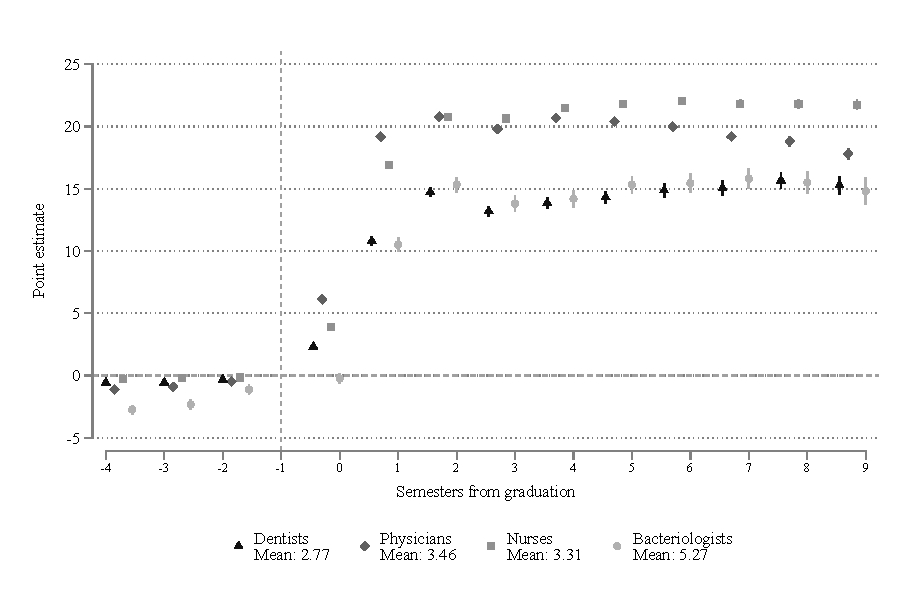
\includegraphics[width=\linewidth]{Figures/Callaway SantAnna/ES_sal_dias_cot_0_female.pdf}
  \caption{Females}
  \label{fig:days_female}
\end{subfigure}%
\begin{subfigure}{.5\textwidth}
  \centering
  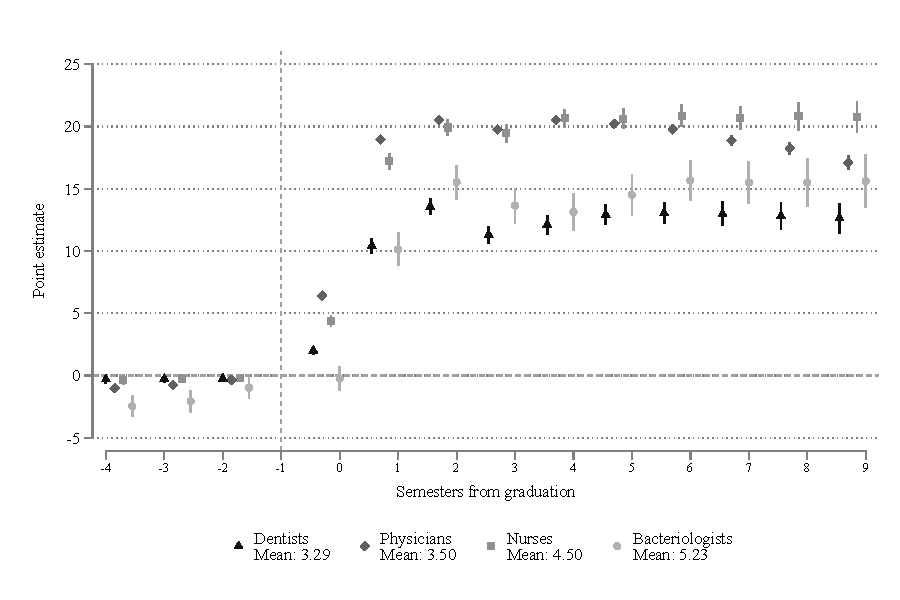
\includegraphics[width=\linewidth]{Figures/Callaway SantAnna/ES_sal_dias_cot_0_male.pdf}
  \caption{Males}
  \label{fig:days_male}
\end{subfigure}
\label{fig:days_gender}
\fnote{\textit{Notes:} Each point represents a coefficient from the \citet{callaway2021difference} estimation. The lines across the coefficients are confidence intervals at the 95\% level. Standard errors are clustered at the individual level. The outcome's mean at the baseline period (-1) for each profession is reported in the legend.}
\end{figure}

\subsubsection{Wages}

\autoref{fig:wage} shows the dynamics of real monthly wages (base year 2018) before and after graduation.\footnote{In 2018, the average exchange rate was 2,956 COP per USD.} In our case, wages are formal earnings, so individuals who did not participate in the formal labor market will have a real monthly wage of zero. In addition, our definition of wages includes the sum of all salaries received in the month when the individual has multiple jobs. Before graduation, all professions had negligible real monthly wages. Upon obtaining their degree, all occupations experience a sharp increase in formal real wages. However, this increase is quite modest in the first semesters, consistent with the initial labor market frictions of the first job \citep{Arellano-Bover2022}. In the semester after graduation ($t=1$), there is a sharp increase in formal earnings associated with the beginning of the social service (SSO) if selected, which is then partially offset with its culmination ($t=3$). The decline in wages after the fifth semester for physicians is likely related to their higher probability of enrollment in postgraduate health programs (as shown below). Despite that, physicians significantly out-earn the other three occupations across our time span.

\begin{figure}[H]
\caption{Real monthly wages}\label{fig:wage}
\centering 
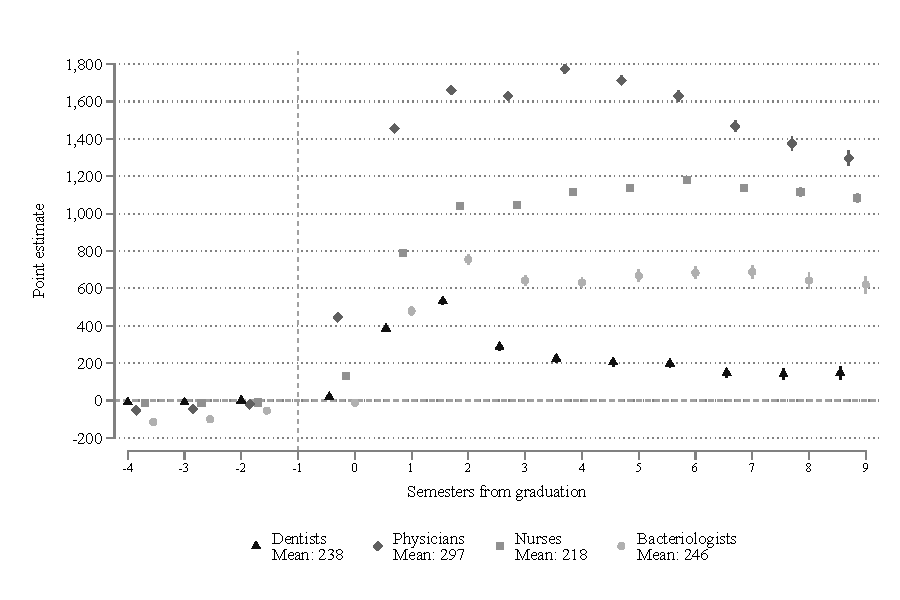
\includegraphics[width=\textwidth]{Figures/Callaway SantAnna/ES_pila_salario_r_0_all.pdf}
\fnote{\textit{Notes:} Each point represents a coefficient from the \citet{callaway2021difference} estimation. Wages are in real Colombian Pesos (base 2018). The lines across the coefficients are confidence intervals at the 95\% level. Standard errors are clustered at the individual level. The outcome's mean at the baseline period (-1) for each profession is reported in the legend.}
\end{figure}

For this particular variable, we highlight the gender gap instead of the separated graphs for each gender (these can be seen in \autoref{fig:wage_gender} in the appendix). We define the gender wage gap for all professions as the difference between the estimated coefficients for males and females in each period and for each profession. \autoref{fig:wage_gap} shows no differences between males and females before obtaining their degree. Nonetheless, even within the first year in the labor market, males out-earn females in medicine and nursing, and the gap increases significantly in the first semesters, stabilizing towards the end of our analysis period. This within-occupation income gap could be partially explained by childbirth \citep{bertrand2010dynamics}, which disproportionately affects women in jobs with lower workplace flexibility \citep{goldin2011cost,goldin2014grand}. In \autoref{fig:pregnancy} in the appendix, we look at the probability of being pregnant for all professions.\footnote{See \autoref{subsec:rips} for a detailed description of how this and other variables are constructed.} We find that pregnancy increases right after graduation and continues increasing until it stabilizes by the end of the analysis period between 2.5 and 4.5 percentage points. While this might explain a share of the gender gap, it is still not sufficient in accounting for the entirety of it. In \autoref{fig:wage_np_gap}, we re-estimate \autoref{fig:wage_gap} but only using women who did not get pregnant in our period of analysis.\footnote{We acknowledge that this exercise restricts the sample using an endogenous variable, not being pregnant. Still, such descriptive statistics show a powerful pattern worth studying further (see \cite{Posso2024gender} for a design-based evaluation in a similar setting).} We find that the gap increases for physicians and nurses in relative terms but is slightly reduced for the rest of the professionals. In addition, our analysis reveals that, in the case of physicians, a small portion of the gap could be attributed to men holding multiple jobs, as shown below. When we focus solely on the salary from the primary job, the gender wage gap diminishes marginally, but the main fact remains (see figure \autoref{fig:wage_max_gap}). 

\begin{figure}[H]
\caption{Real monthly wage (gender gap)}\label{fig:wage_gap}
\centering 
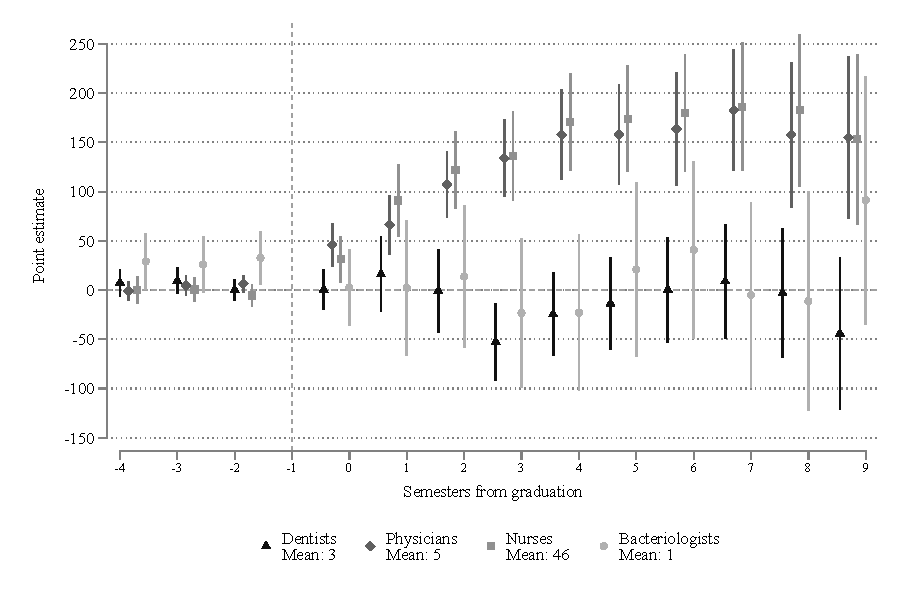
\includegraphics[width=\textwidth]{Figures/Callaway SantAnna/ES_pila_salario_r_0_gap.pdf}
\fnote{\textit{Notes:} Each point and confidence interval comes from a difference-in-means Welch t-test from the \citet{callaway2021difference} estimations. Wages are in real Colombian Pesos (base 2018). The confidence intervals are at the 95\% level. The gap at the baseline period (-1) for each profession is reported in the legend. Positive values indicate a gap in favor of men.}
\end{figure}

\subsubsection{Type and number of jobs}

One key characteristic of the Colombian labor market is that many workers are hired as self-employees. This is even more important for health professionals \citep{Procuraduria2020}. Such types of contracts are associated with either lower quality conditions\footnote{For instance, short-term contracts with no additional benefits or less occupational hazards protection.} or professionals with their own businesses, such as a dentist with a private practice.\footnote{As explained in \autoref{sec:context}, these contracts may be used to avoid taxes by under-reporting income since each person reports their earnings. In Spain, \citet{garcia2023dual} find lower returns in fixed-term contracts compared to permanent contracts.} When considering the probability of being self-employed, \autoref{fig:self} shows that it increases for all four professions by around 15-20 percentage points in the second semester after undergraduate graduation. This probability slowly declines for all professionals, except dentists, who remain stable at 27-30 percentage points. 

\begin{figure}[H]
\caption{Probability of being self-employed}\label{fig:self}
\centering 
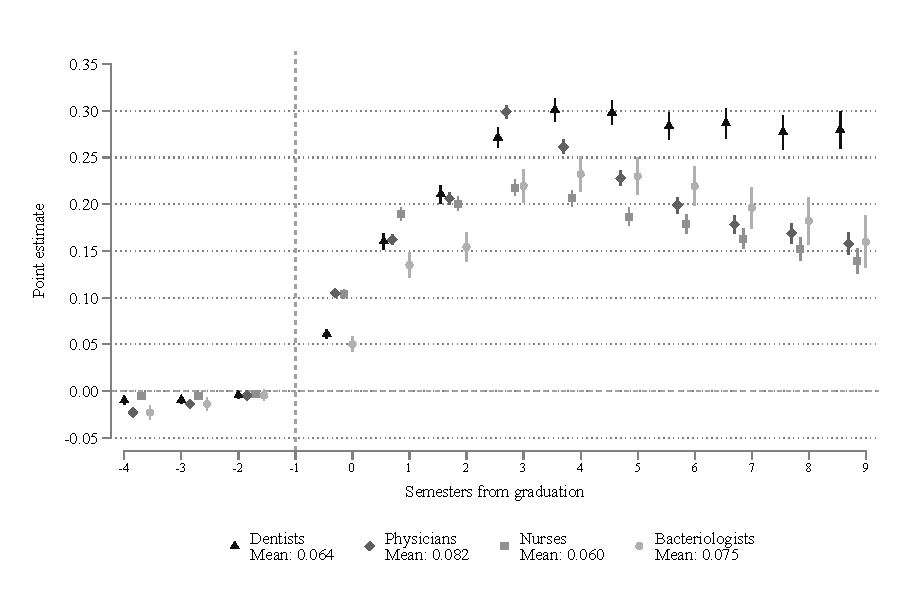
\includegraphics[width=\textwidth]{Figures/Callaway SantAnna/ES_pila_independientes_all.pdf}
\fnote{\textit{Notes:} Each point represents a coefficient from the \citet{callaway2021difference} estimation. The lines across the coefficients are confidence intervals at the 95\% level. Standard errors are clustered at the individual level. The outcome's mean at the baseline period (-1) for each profession is reported in the legend.}
\end{figure}

The real wage results in \autoref{fig:wage} showed that dentists report the lowest earnings. One potential explanation for this result is that self-employed workers in Colombia report their income in a setting where the fiscal capacity is limited. For these individuals, the contribution base is 40\% of their gross income and should be between the monthly minimum wage and any level of earnings above it.\footnote{See \autoref{subsec:pila} for a detailed discussion on this.} Social security payments are usually around 28.5\% of the reported income. As \citet{kleven2013using} showed, this type of discontinuities in the choice sets of individuals (like the minimum wage here) introduces a behavioral incentive for moving from a region above the minimum wage to a point just at the minimum wage, creating a bunching in the distribution of reporting earnings at the minimum wage; a fact that we observe in Colombia and in particular for dentists.

Across professions, there are no significant gender differences in the probability of being self-employed, except for dentists. \autoref{fig:self_gender} shows that there are not many differences between professions for males, and dentists also show a decreasing trend eventually. However, female dentists show a stark difference that accounts for what was seen in the general pattern. They are more likely to be self-employed than other professionals, and this remains stable over time.

\begin{figure}[H]
\centering
\caption{Probability of being self-employed by gender}
\begin{subfigure}{.5\textwidth}
  \centering
  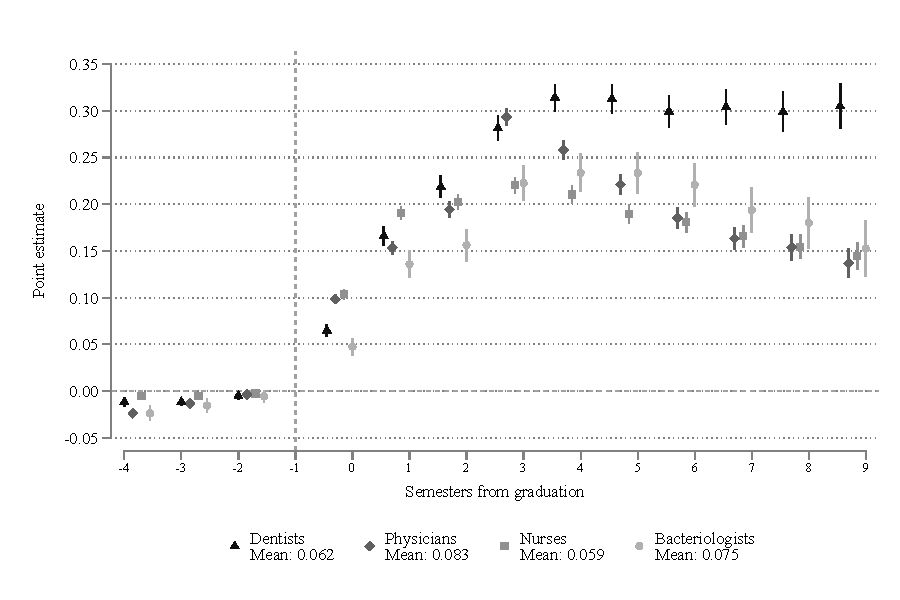
\includegraphics[width=\linewidth]{Figures/Callaway SantAnna/ES_pila_independientes_female.pdf}
  \caption{Females}
  \label{fig:self_female}
\end{subfigure}%
\begin{subfigure}{.5\textwidth}
  \centering
  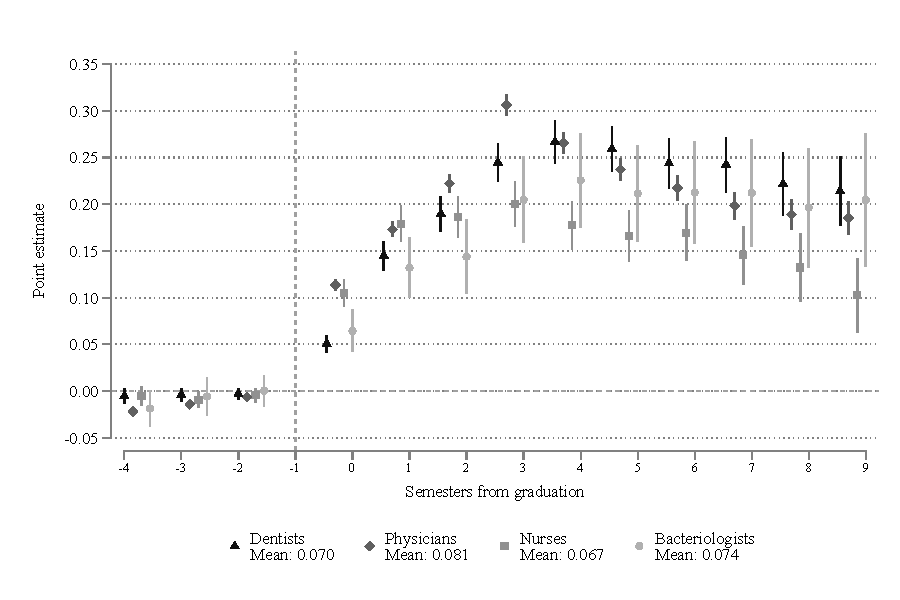
\includegraphics[width=\linewidth]{Figures/Callaway SantAnna/ES_pila_independientes_male.pdf}
  \caption{Males}
  \label{fig:self_male}
\end{subfigure}
\label{fig:self_gender}
\fnote{\textit{Notes:} Each point represents a coefficient from the \citet{callaway2021difference} estimation. The lines across the coefficients are confidence intervals at the 95\% level. Standard errors are clustered at the individual level. The outcome's mean at the baseline period (-1) for each profession is reported in the legend.}
\end{figure}

Another important feature of the health professionals' labor market is that many professionals usually have multiple jobs. \autoref{fig:numberjobs} shows the trajectory for the probability of having multiple (simultaneous) jobs. While bacteriologists and dentists do not show high levels of this outcome after graduation, nurses, and especially physicians, do. In all cases, we observe an inverted u-pattern through time, although it is significantly more pronounced for physicians. The marked inverse u-pattern observed in physicians may be associated with the beginning of graduate school, as will later be shown. 

\begin{figure}[H]
\caption{Probability of having multiple jobs}\label{fig:numberjobs}
\centering 
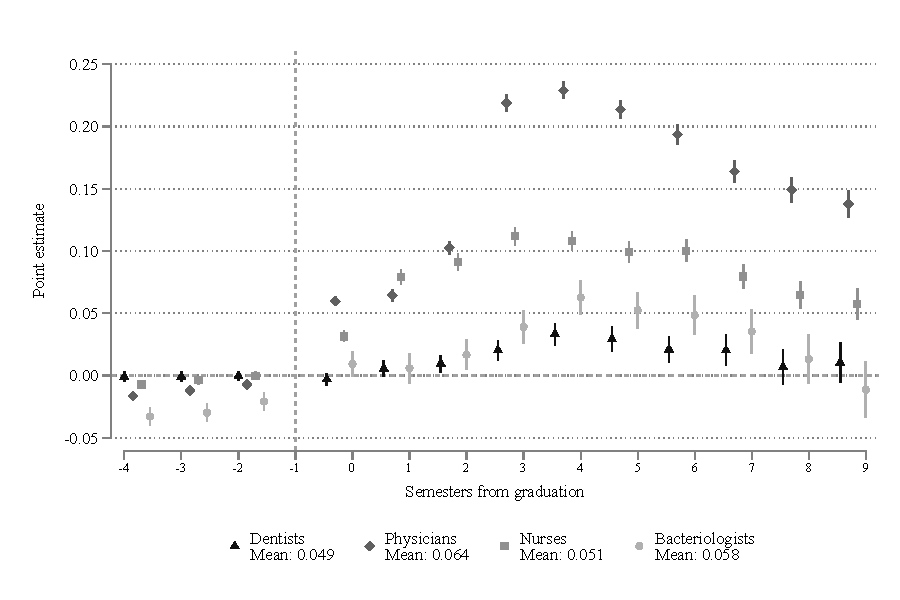
\includegraphics[width=\textwidth]{Figures/Callaway SantAnna/ES_p_cotizaciones_0_all.pdf}
\fnote{\textit{Notes:} Each point represents a coefficient from the \citet{callaway2021difference} estimation. The lines across the coefficients are confidence intervals at the 95\% level. Standard errors are clustered at the individual level. The outcome's mean at the baseline period (-1) for each profession is reported in the legend.}
\end{figure}

There do not appear to be many differences between male and female professionals for nurses and bacteriologists (see \autoref{fig:numberjobs_gender}). However, when looking at the gender differences between physicians and dentists (see \autoref{fig:numberjobs_gap} in the appendix for the gap), there are some interesting results. The probability of having multiple jobs is higher for male physicians, who eventually have an around four percentage points higher probability of having simultaneous jobs than their female counterparts nine semesters after graduating. Since our measure of wages is the sum of all salaries when the individual has multiple jobs, this accounts for a share of the gender wage gap previously analyzed.\footnote{When we only take into account the main wage across jobs as an outcome, the gender gap follows the same pattern (see \autoref{fig:wage_max_gap} in the appendix). This entails that, the number of jobs and childbirth explains a small share of the wage gap} Male dentists, on the other hand, have a lower probability of having simultaneous jobs.

\begin{figure}[H]
\centering
\caption{Probability of having multiple jobs by gender}
\begin{subfigure}{.5\textwidth}
  \centering
  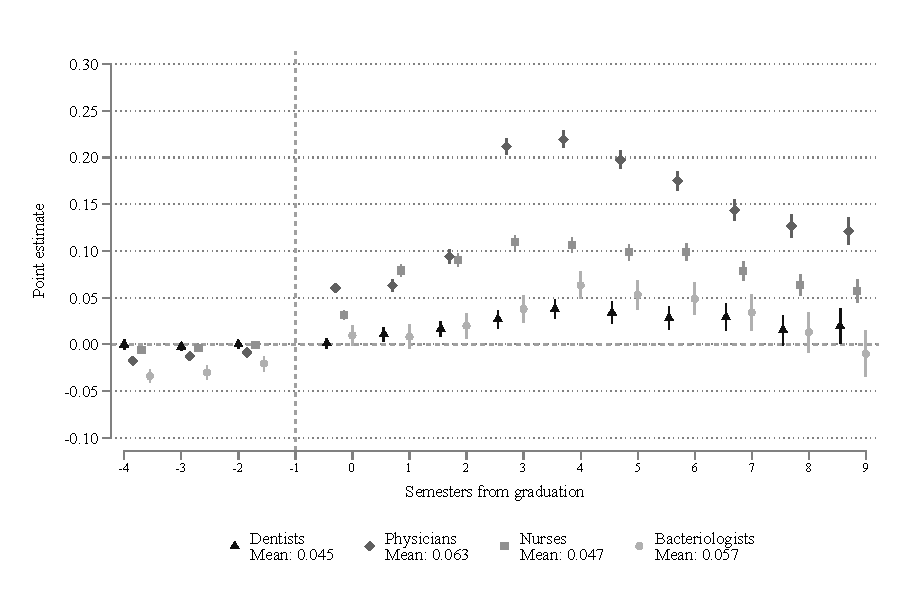
\includegraphics[width=\linewidth]{Figures/Callaway SantAnna/ES_p_cotizaciones_0_female.pdf}
  \caption{Females}
  \label{fig:numberjobs_female}
\end{subfigure}%
\begin{subfigure}{.5\textwidth}
  \centering
  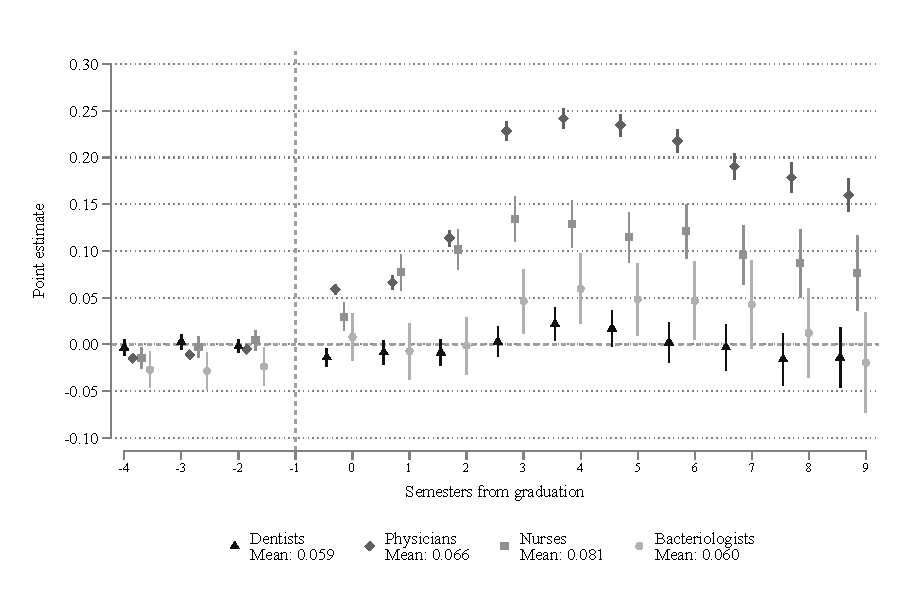
\includegraphics[width=\linewidth]{Figures/Callaway SantAnna/ES_p_cotizaciones_0_male.pdf}
  \caption{Males}
  \label{fig:numberjobs_male}
\end{subfigure}
\label{fig:numberjobs_gender}
\fnote{\textit{Notes:} Each point represents a coefficient from the \citet{callaway2021difference} estimation. The lines across the coefficients are confidence intervals at the 95\% level. Standard errors are clustered at the individual level. The outcome's mean at the baseline period (-1) for each profession is reported in the legend.}
\end{figure}

\subsubsection{Health graduate school}

An interesting feature of the social security system in Colombia is that it is mandatory for all full-time graduate health students and medical residents, even if not formally employed, to contribute to the social security system through PILA \citep{Minsalud}. This regulation applies mainly to medical residencies and dental postgraduate programs where there is contact with patients. This allows us to measure enrollment trajectories in health postgraduate programs for physicians and dentists. Nonetheless, it is not a good measure for bacteriologists and nurses or other types of postgraduate programs such as a Ph.D. or a master's in administration or science. Thus, in this section, we only focus on postgraduate trajectories for physicians and dentists.

As mentioned in \autoref{sec:context}, postgraduate degrees in health-related areas are particularly important for these occupations, given their limited availability and high returns. \autoref{fig:postgrad} shows the results on access to these types of degrees. The pre-treatment coefficients are mechanically set to zero since an individual may not enroll in a postgraduate program before obtaining the undergraduate degree \citep{Minsalud2007,Minsalud2011}. Physicians and dentists show a similar increasing pattern in the first two years after graduation (t=4). After that, the effect is stabilized for dentists but continues to increase for physicians up to four and a half years after graduation. In period t=9, more than 14 percent of physicians are enrolled in a postgraduate program in health, while only above seven percent of dentists are.

It is important to note that the pattern in postgraduate enrollment coincides with the observed decline in wages, type of contract, and multiple jobs for physicians. Hence, postgraduate school should be a key factor in explaining the labor market trajectories of physicians.\footnote{In a separate research agenda, we study the consequences of postgraduate programs for physicians.} 


\begin{figure}[H]
\caption{Probability of enrollment in a health-related postgraduate program}\label{fig:postgrad}
\centering 
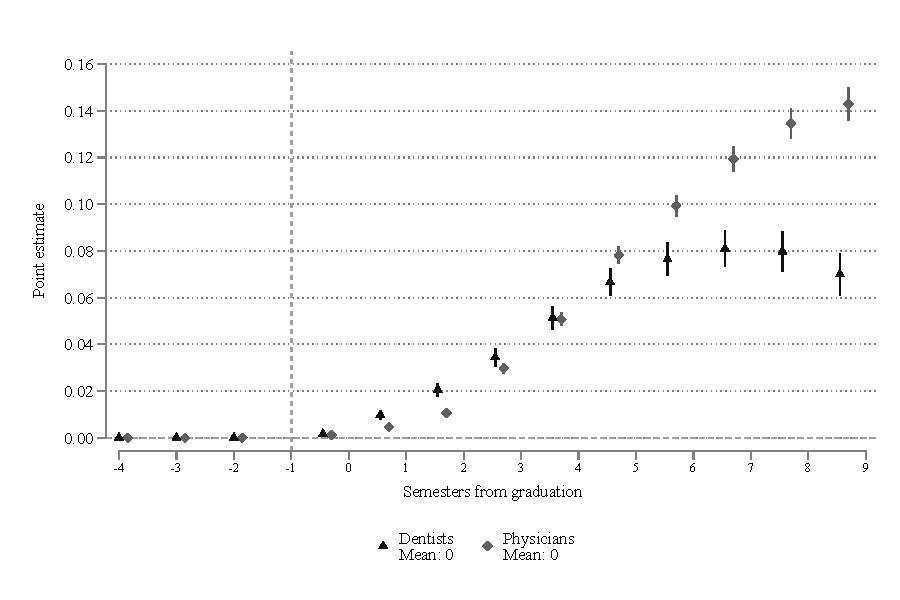
\includegraphics[width=\textwidth]{Figures/Callaway SantAnna/ES_posgrado_salud_all.pdf}
\fnote{\textit{Notes:} Each point represents a coefficient from the \citet{callaway2021difference} estimation. The lines across the coefficients are confidence intervals at the 95\% level. Standard errors are clustered at the individual level. The outcome's mean at the baseline period (-1) for each profession is reported in the legend.}
\end{figure}

The results for each gender are presented in \autoref{fig:postgrad_gender} in the appendix. Like in the wages subsection, we also focus on the gender gap for physicians and dentists, measured as the difference between the estimated coefficients for males and females in each period and profession (see \autoref{fig:postgrad_gap}). Results show that even within the first year after graduation, male physicians are more likely to enroll in a health postgraduate program than females. The gap for physicians is around one percentage point from period t=3 to period t=7, which represents between 11.6\% and 26.7\% of the increase in male enrollment seen in \autoref{fig:postgrad_gender}. In the case of dentists, the gap is only significant between periods t=3 and t=5, and it is similar to physicians in relative terms.

This result raises a new question: does the graduate enrollment gap affect the wage gap? To answer this, we re-estimated two variations of \autoref{fig:wage_gap}, presenting both estimates in \autoref{fig:wage_gap_pos}. First, we only include professionals who never enrolled in graduate studies. Then, we restrict the sample to professionals who started graduate studies within our time span (eventually enrolled). Since \autoref{fig:wage_gap} compares the salary of all professionals, the gap may be skewed due to more men entering graduate school and having different working conditions than general practitioners. We find that gaps for never-enrolled professionals are almost indistinguishable from \autoref{fig:wage_gap}, although decreasing in the long run. On the other hand, eventually-enrolled physicians increased their gap dramatically in the latter years.

\begin{figure}[H]
\caption{Probability of enrollment in a health-related postgraduate program (gender gap)}\label{fig:postgrad_gap}
\centering 
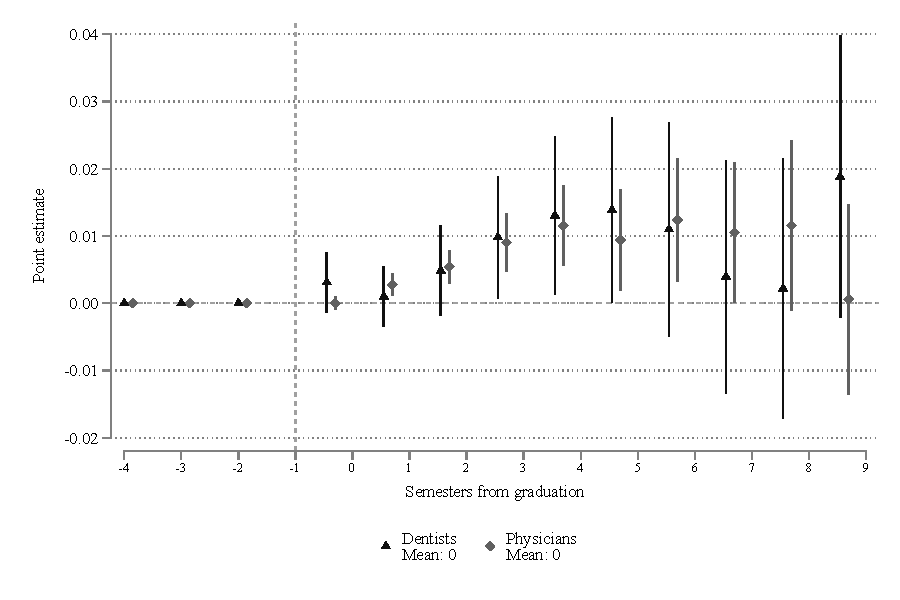
\includegraphics[width=\textwidth]{Figures/Callaway SantAnna/ES_posgrado_salud_gap.pdf}
\fnote{\textit{Notes:} Each point and confidence interval comes from a difference-in-means Welch t-test from the \citet{callaway2021difference} estimations. The confidence intervals are at the 95\% level. The gap at the baseline period (-1) for each profession is reported in the legend. Positive values indicate a gap in favor of men.}
\end{figure}

This result is related to what is referred to as the “glass ceiling” or the fact that women are underrepresented in the upper part of the earnings distribution or top positions in society \citep{goldin2014grand}. In the particular case of health professionals, the top positions and salaries are strictly associated with the possibility of access to postgraduate education. Our methods allow us to provide a setting where innate talent, or other fixed characteristics, are isolated at the beginning of the professional career. Still, we observe differences between men and women at the beginning of their careers that cannot be explained by access to postgraduate education. 

\subsection{Health trajectories \label{sec:rips}}

The previous section showed that health professionals have relatively high returns on their employment outlooks after bachelor studies. It also shows how important labor and education conditions are for shaping labor market outcomes. Overall, physicians are the professionals who enjoy the most benefits, as expected, but this is also related to the amount of work they do. Along with these high economic returns, the literature has typically focused on tuition \citep{altonji2018costs} to look at net returns, with more recent studies also focusing on time costs \citep{altonji2023effects}. However, there is limited evidence on the associated health costs that might be correlated with higher monetary returns \citep{heckman2018returns}. This subsection presents the trajectories associated with these professionals' health outcomes as a proxy for non-monetary returns. 

We focus on two outcomes: bad health outcomes and mental health diagnoses. The first one tries to capture the trajectories of bad health events after the beginning of their professional career. There is evidence that the nature of the work carried out by health care professionals is associated with higher health risks \citep{mohanty2019health,kobo2023causes}. In addition, Colombian labor regulations require that all formal workers be protected against potential occupational hazards or risks associated with the work performed. The risk classification varies between 1 and 5, with 5 being the highest risk. Most workers are level 1.\footnote{Low-risk professionals are those categorized as level 1 and 2; by January 2022, they comprised 68\%. Level 3 includes 14\%, while levels 4 and 5 include 8.5\% and 9.9\% respectively} High-risk occupations comprise levels 3 to 5. Given the constant interaction with humans, body fluids, bio-mechanical risks, or activities related to handling chemicals, diagnostic imaging, radio-pharmaceuticals, and nuclear medicine, health professionals are usually categorized as high-risk occupations \citep{Ministeriodetrabajoyseguridadsocial}. Using our claim health data (RIPS), we measure bad health events as either an emergency room (ER) visit or a hospitalization \citep{hansagi2001frequent}. Such events are associated with a service that indicates a situation of poor health, where a person's life is at risk and requires immediate attention (ER visits) or prolonged direct care (hospitalization).\footnote{According to Decree 412 of 1992, an Emergency corresponds to alterations in the physical and/or mental integrity of a person caused by trauma or by an illness that generates a demand for immediate and effective medical attention aimed at reducing the risks of disability and death}

The second outcome focuses on mental health diagnoses. There is evidence of the prevalence of mental illnesses and burnout in health professionals \citep{lai2020factors,young2021health,simon2022analisis,gold2013details,johnson2018mental,shanafelt2017executive, west2020resilience}. The demanding nature of the occupation exposes health workers to a higher risk of developing negative mental states such as depression, anxiety, and stress \citep{ghazwin2016association,huang2018risks,maharaj2019prevalence}. These health problems could be considered an additional cost that health workers assume and is usually hard to measure.

However, mental health problems in the healthcare workforce do not occur at the beginning of their working life. There is extensive literature that supports that students in health programs, even from the selection process, may be particularly vulnerable to mental illness due to feelings of rigidity, perfectionism, and excessive devotion to work \citep{mihailescu2019scoping,parsons2020evidence,afshar2022perceived,ferrel2011depresion}. Yet this situation may change upon graduation. Individuals may feel less pressure after exiting their bachelor programs and may experience a reduction in the probability of a mental disorder from this improved feeling of comfort. Or they could be reluctant to get professional help since a diagnosis of mental illness may create a stigma associated with their ability to practice their profession.


\subsubsection{Emergency Room (ER) Visits and Hospitalizations}
\autoref{fig:er} shows the trajectories for each of the four health occupations in the probability of having an ER visit. On average, nurses, physicians, and bacteriologists are the professionals with the largest increase in the probability of an ER visit after obtaining their degree. Nurses are around 54\% more likely to go to the ER one year after graduation relative to the period just before graduation. Such effects are persistent even after four years. For dentists, we do not observe any significant change after graduation. These results are interesting because they show professionals' high heterogeneity in health risk.

\begin{figure}[H]
\caption{Probability of going to the ER}\label{fig:er}
\centering 
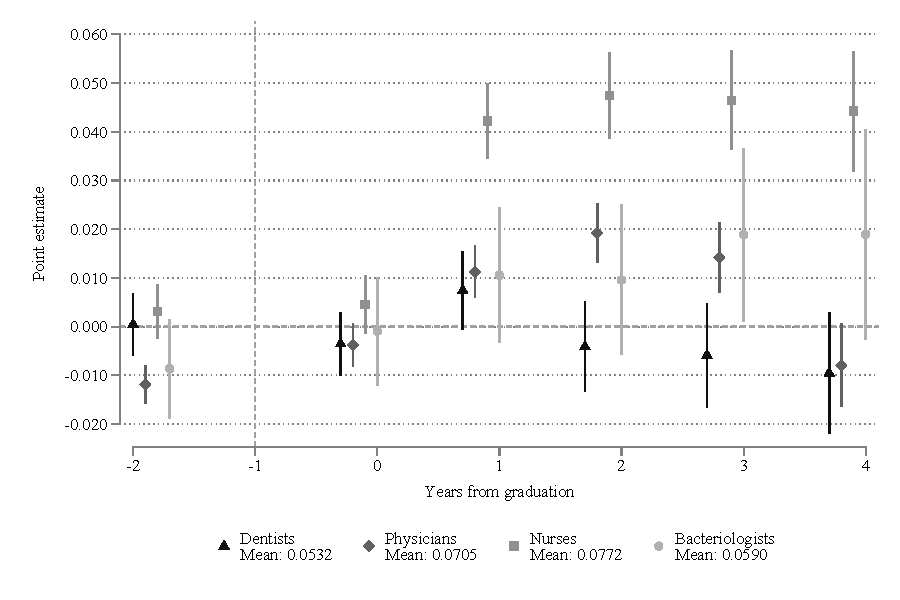
\includegraphics[width=\textwidth]{Figures/Callaway SantAnna/ES_urg_all.pdf}
\fnote{\textit{Notes:} Each point represents a coefficient from the \citet{callaway2021difference} estimation. The lines across the coefficients are confidence intervals at the 95\% level. Standard errors are clustered at the individual level. The outcome's mean at the baseline period (-1) for each profession is reported in the legend.}
\end{figure}

When dividing the results by gender (see \autoref{fig:er_gender}), we see that the increase in ER visits for nurses and physicians happens for both men and women. However, although noisier, the estimates show a lower probability for male dentists a few years after graduation. Overall, men and women have no major differences (see \autoref{fig:er_gap} in the appendix). We also check whether the increase in probability for women is driven by pregnancy by estimating the same regressions on the probability of going to the ER for something unrelated to pregnancy. Results are virtually the same, highlighting that pregnancy does not drive the higher ER access for women (see \autoref{fig:er_np_female} in the appendix). 

\begin{figure}[H]
\centering
\caption{Probability of going to the ER by gender}
\begin{subfigure}{.5\textwidth}
  \centering
  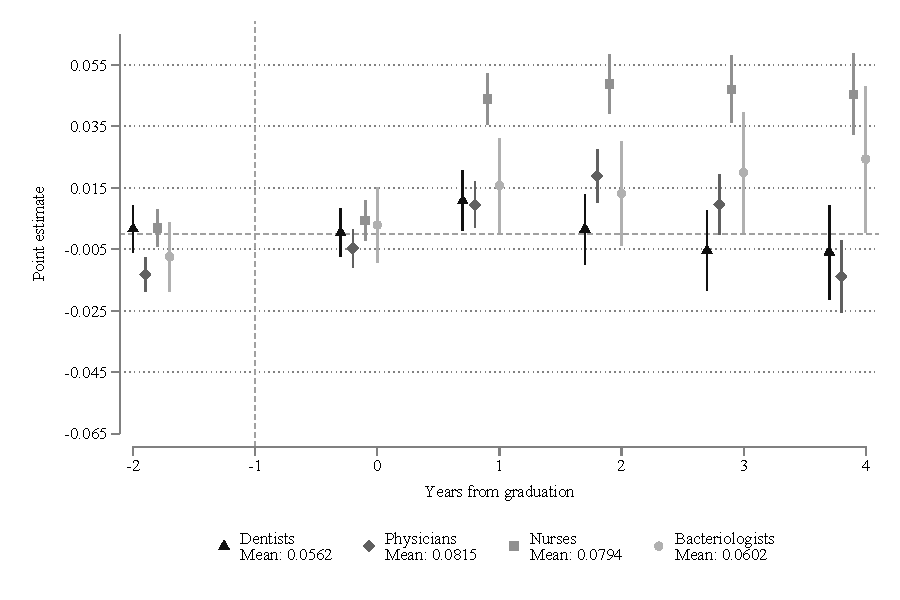
\includegraphics[width=\linewidth]{Figures/Callaway SantAnna/ES_urg_female.pdf}
  \caption{Females}
  \label{fig:er_female}
\end{subfigure}%
\begin{subfigure}{.5\textwidth}
  \centering
  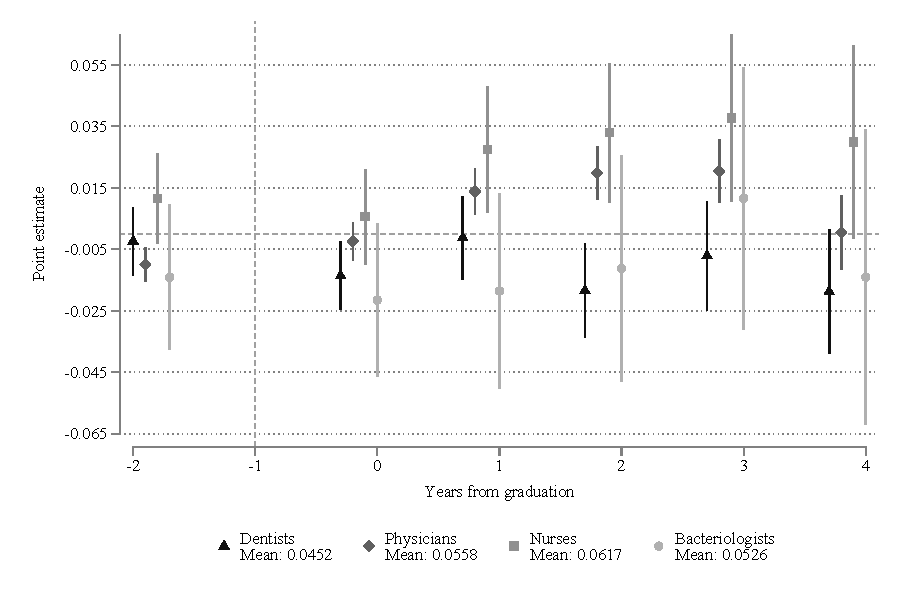
\includegraphics[width=\linewidth]{Figures/Callaway SantAnna/ES_urg_male.pdf}
  \caption{Males}
  \label{fig:er_male}
\end{subfigure}
\label{fig:er_gender}
\fnote{\textit{Notes:} Each point represents a coefficient from the \citet{callaway2021difference} estimation. The lines across the coefficients are confidence intervals at the 95\% level. Standard errors are clustered at the individual level. The outcome's mean at the baseline period (-1) for each profession is reported in the legend.}
\end{figure}

We then focus on the probability of being hospitalized in \autoref{fig:hosp}. Shockingly, all professionals are more likely to be hospitalized one year after graduation, and this probability increases over time for all professionals, particularly nurses and bacteriologists. While relative to the pre-graduation period, dentists are around 77\% more likely to be hospitalized four years after graduation, physicians and nurses are 118\% and 221\% more likely, respectively.\footnote{The relative effect is over 328\% for bacteriologists, but the pre-graduation mean is much lower, and the point estimate is much noisier.} This might be indicative of harsher job conditions in the nursing field.

\begin{figure}[H]
\caption{Probability of hospitalization}\label{fig:hosp}
\centering 
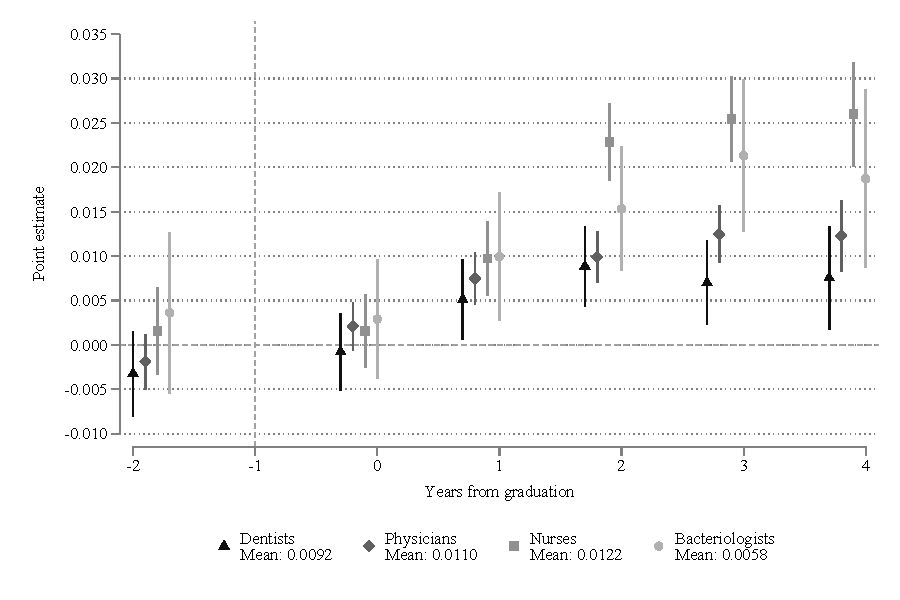
\includegraphics[width=\textwidth]{Figures/Callaway SantAnna/ES_hosp_all.pdf}
\fnote{\textit{Notes:} Each point represents a coefficient from the \citet{callaway2021difference} estimation. The lines across the coefficients are confidence intervals at the 95\% level. Standard errors are clustered at the individual level. The outcome's mean at the baseline period (-1) for each profession is reported in the legend.}
\end{figure}

Separating these results by gender shows an interesting heterogeneity (see \autoref{fig:hosp_gender}). The effects are more pronounced for women across professions, but for bacteriologists, the effects are stronger. When estimating the gender gap within occupations, \autoref{fig:hosp_gap} in the appendix shows that for all professions but bacteriology, women's coefficients are larger than men's. Nonetheless, such a gap is partially explained by childbirth, which usually requires hospitalization. Just as in ER visits, we discount the effect of pregnancy from women's estimates. While overall hospitalizations are an important health risk among professionals, the gender gap against women within occupations is only present for nurses and dentists (see \autoref{fig:hosp_np_gap} in the appendix). 

\begin{figure}[H]
\centering
\caption{Probability of hospitalization by gender}
\begin{subfigure}{.5\textwidth}
  \centering
  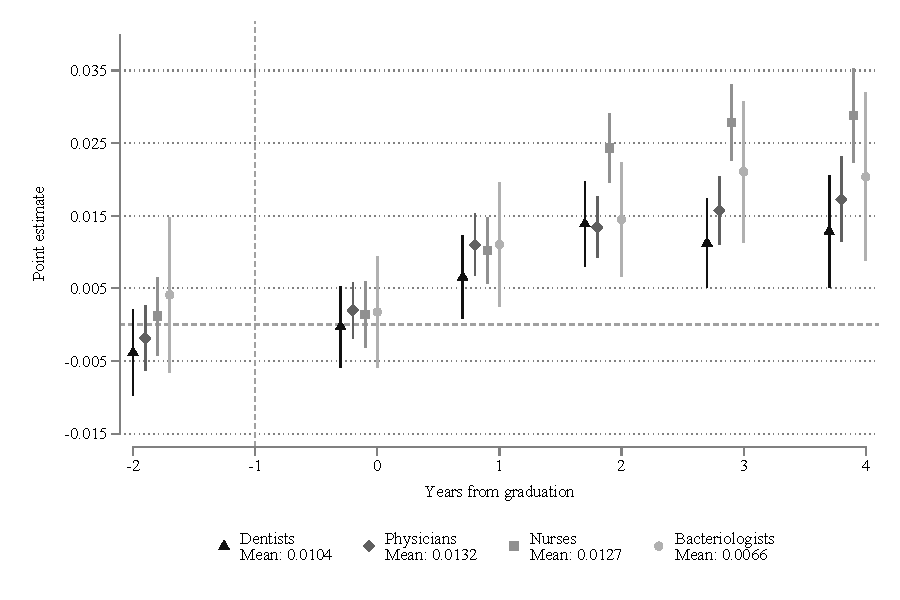
\includegraphics[width=\linewidth]{Figures/Callaway SantAnna/ES_hosp_female.pdf}
  \caption{Females}
  \label{fig:hosp_female}
\end{subfigure}%
\begin{subfigure}{.5\textwidth}
  \centering
  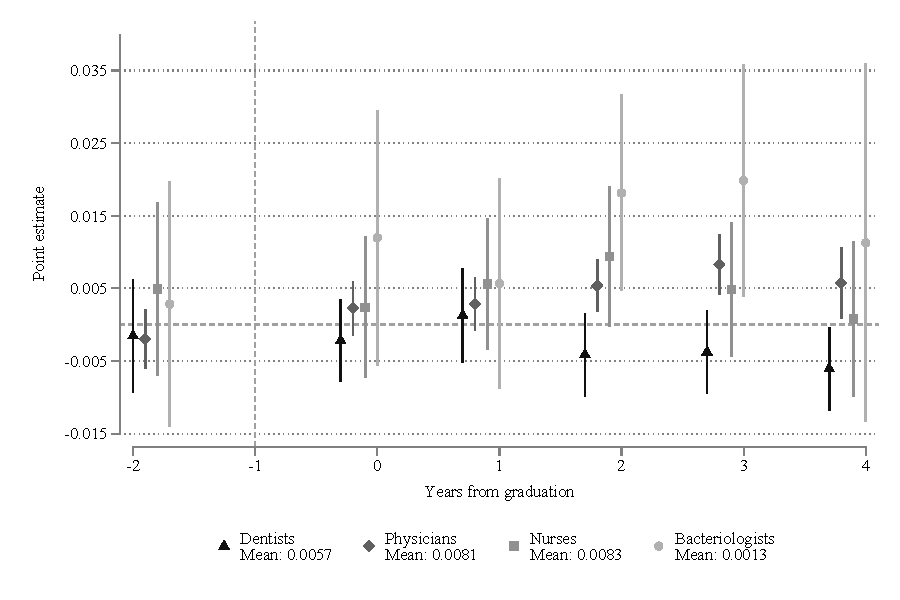
\includegraphics[width=\linewidth]{Figures/Callaway SantAnna/ES_hosp_male.pdf}
  \caption{Males}
  \label{fig:hosp_male}
\end{subfigure}
\label{fig:hosp_gender}
\fnote{\textit{Notes:} Each point represents a coefficient from the \citet{callaway2021difference} estimation. The lines across the coefficients are confidence intervals at the 95\% level. Standard errors are clustered at the individual level. The outcome's mean at the baseline period (-1) for each profession is reported in the legend.}
\end{figure}

\subsubsection{Mental health diagnosis}
Finally, we examine the trajectories of mental health. Our health claim data measures medical diagnoses of mental illnesses rather than episodes. Usually, in the diagnostic process, taking the time and effort to get an accurate diagnosis helps determine the appropriate treatment. Once determined, most mental illnesses are long-term conditions.\footnote{Our main outcome measures any mental health diagnosis. This is because sometimes, as new episodes appear, physicians update the diagnosis and treatment. Our results show that the main illnesses affecting health professionals are depression and anxiety.} Here, we focus on measuring prevalence rather than incidence. 


As outlined in \autoref{subsec:rips}, we measure prevalence (following medical literature)\footnote{Prevalence is commonly defined in medical literature as the number of existing cases at the beginning of the period studied, plus the new cases developed during the interval \citet{gbd2022global}.} by defining a mental condition as the accumulation of the episodes mentioned above. This implies that from the moment individuals receive a mental illness diagnosis, it is assumed that they will continue to have this condition from this point onwards. Intrinsically, these estimates compare the existence of a mental condition in graduated professionals with respect to those who have not yet graduated. Thus, coefficients in \autoref{fig:mental_forever} can be interpreted as the probability of having a mental condition after graduation relative to the final stage of their bachelor studies.

Results show that dentists and nurses increase their prevalence of having a mental condition by just over one percentage point by the fourth year after graduation, representing a relative effect of 35\% and 26\%, respectively. On the other hand, physicians decrease their probability by almost 1.5 percentage points after four years, consistent with a relative effect of 37\% reduction. One possible explanation for the latter result is the demanding nature of undergraduate programs in medicine. Although their work can be as stressful as their career, physicians face fairly promising job prospects once they graduate, as shown in \autoref{sec:pila}. Thus, these professionals may be reducing the prevalence of reported mental illnesses once they graduate, not necessarily because they are healthier, but because they can face these difficulties from a much more comfortable position. An alternative reasonable explanation is that physicians are avoiding revealing their mental conditions as a way to steer clear of negative prejudices. Understanding the reasons for this result is beyond the scope of this paper. 

\begin{figure}[H]
\caption{Probability of having a mental condition}\label{fig:mental_forever}
\centering 
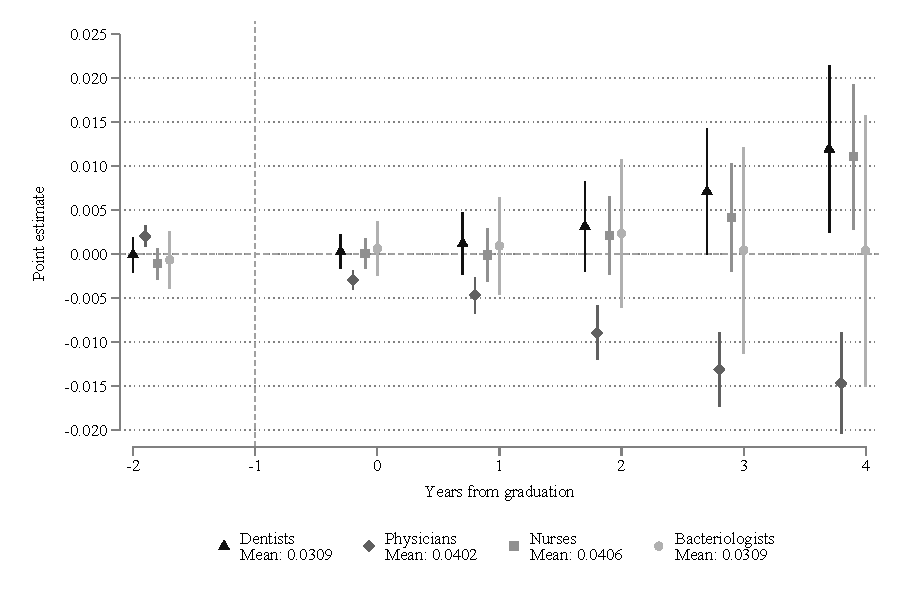
\includegraphics[width=\textwidth]{Figures/Callaway SantAnna/ES_service_mental_forever_all.pdf}
\fnote{\textit{Notes:} Each point represents a coefficient from the \citet{callaway2021difference} estimation. The lines across the coefficients are confidence intervals at the 95\% level. Standard errors are clustered at the individual level. The outcome's mean at the baseline period (-1) for each profession is reported in the legend.}
\end{figure}

\autoref{fig:mental_forever} and \autoref{fig:mental_forever_gap} show that most professionals have similar trajectories regardless of gender. However, the case of nurses is particularly different. While women's probability of mental illness increases significantly by 36\%, men's decreases by the same proportion, although their results are too noisy to be precise.

\begin{figure}[H]
\centering
\caption{Probability of having a mental condition by gender}
\begin{subfigure}{.5\textwidth}
  \centering
  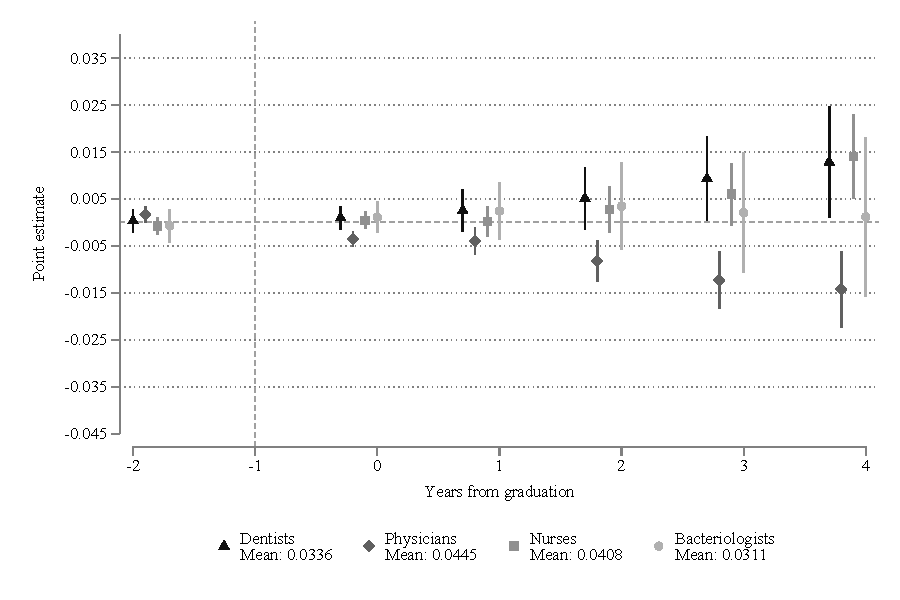
\includegraphics[width=\linewidth]{Figures/Callaway SantAnna/ES_service_mental_forever_female.pdf}
  \caption{Females}
  \label{fig:mental_forever_female}
\end{subfigure}%
\begin{subfigure}{.5\textwidth}
  \centering
  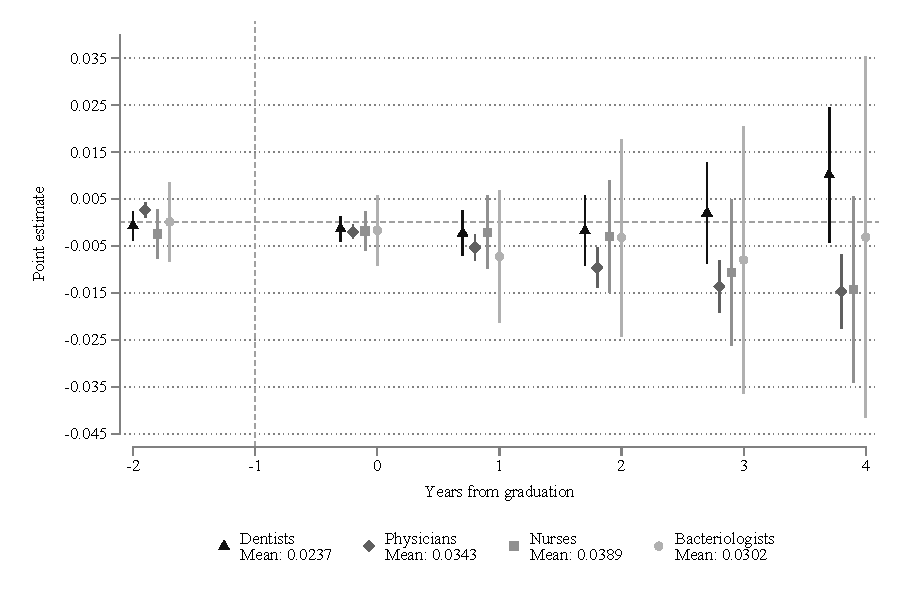
\includegraphics[width=\linewidth]{Figures/Callaway SantAnna/ES_service_mental_forever_male.pdf}
  \caption{Males}
  \label{fig:mental_forever_male}
\end{subfigure}
\label{fig:mental_forever_gender}
\fnote{\textit{Notes:} Each point represents a coefficient from the \citet{callaway2021difference} estimation. The lines across the coefficients are confidence intervals at the 95\% level. Standard errors are clustered at the individual level. The outcome's mean at the baseline period (-1) for each profession is reported in the legend.}
\end{figure}


%%%%%%%%%%%%%%%%%%%%%%%%%%%%%%%%%%%%%%%%%%%%%%%%%%%%
\section{Conclusion} \label{sec:conclusion}

In this paper, we study the initial trajectories of healthcare professionals in Colombia's labor market, graduate school, and health. We take advantage of Colombian administrative data that allow us to capture the entire population of recently graduated professionals in bacteriologists, nurses, physicians, and dentists. Our data quality enables us to track these professionals before and after graduation from college across multiple outcomes. To accomplish this, we exploit the graduation dates of individuals in a staggered event study framework to determine their working and health conditions relative to that moment.

Overall, we observe that the professional trajectories are heterogeneous by type of professional and gender. We document significant monetary returns in their early years for all professionals. Trajectories also depend on demand-side labor market institutions that affect working conditions (non-monetary incentives), like the types of contracts offered, the number of jobs available, and health-related postgraduate programs. Some professions, like dentistry, are more prone to self-employment, while others are likelier to have multiple jobs, like physicians. Nonetheless, we find significant gender wage and postgraduate access gaps for physicians and nurses that start upon graduation and are sustained over time. 

Moreover, there are also large heterogeneities across professions in health trajectories. While nurses and physicians are more likely to go to the ER after graduation, all professionals face higher odds of being hospitalized, with women, especially nurses, being disproportionately affected by this. 

Meanwhile, the prevalence of mental health diagnoses increases for nurses and dentists, while it shows a reduction for physicians. Assuming that mental illness may be a lifelong condition, human talent in these former professions may be facing relatively worrisome conditions.

Our study is the first to provide evidence on Colombia's healthcare workers' trajectories. Additionally, using a rigorous empirical framework, it is one of the few papers to combine the labor market, postgraduate education, and health outcomes in the early years of a professional career. These are particularly relevant since they may affect the recruitment and retention of healthcare personnel. Thus affecting workers' supply. In this context, our paper might provide purposeful empirical evidence on work and health conditions to guide the actions of policymakers, who have been under increased scrutiny following the COVID-19 pandemic.

\newpage
\bibliographystyle{apacite}
\bibliography{references}

\newpage
\appendix
\counterwithin{figure}{section}
\counterwithin{table}{section}

\section{Data construction appendix \label{sec:data_appendix}}

In this section, we outline our main approach to data construction. As such, we provide a detailed description of the restrictions we placed on our datasets and how we constructed the time-to-event and outcome variables. Additionally, we explain how the rest of the Ministry of Health and Social Protection's data were matched to create a unique individual-level longitudinal dataset with all the information on the formal labor market, graduate education and health outcomes for the selected healthcare workers in the country.


\subsection{ReTHUS}

We begin by restricting the ReTHUS data to the four occupations requiring the SSO: bacteriologists, physicians, nurses, and dentists. We also keep observations for individuals who graduated from only one major. Multiple-degree professionals are not considered to maintain consistency in our estimations. Additionally, we focus on people who obtained their degree between 2011 and 2017 to see enough periods pre- and post-graduation. Overall, these restrictions leave us with a total sample size of \samplerethus.

We call this our main sample since it contains all legally registered professionals in the country in our selected occupations. The main variables gathered from this source are occupation code, graduation dates, gender, and \textit{personabasicaid}. The first one is a categorical variable indicating each individual's occupation in the following way: P01 refers to bacteriologists, P03 to nurses, P07 to physicians, and P09 to dentists. Graduation dates are when the person received the undergraduate and postgraduate degrees, respectively. The former will be crucial to identify cohorts in the \citet{callaway2021difference} estimation. The gender variable will allow us to examine potential heterogeneities between males and females. As for \textit{personabasicaid}, this is an anonymized personal identifier that tracks individuals across the Ministry of Health and Social Protection's datasets.

\subsection{PILA \label{subsec:pila}}

To construct our labor market outcomes, we merge our main sample with the \textit{Planilla Integrada de Liquidación de Aportes} using the \textit{personabasicaid}. PILA contains all the monthly social security payments made by all formal workers in the country. We have access to these data from 2008 to August 2022. The dataset construction works in the following way. First, we call the year-month PILA dataset and merge it with our main sample, only keeping matched observations. Using the type of contributor code, we identify whether an individual is a dependent or self-employed worker and whether the person is enrolled in a health-related postgraduate course. The specific codes are shown in \autoref{tab:codes}.

\begin{table}[H]
  \centering
  \caption{PILA contributor codes}
  \begin{threeparttable}
    \begin{tabular}{llc}
    \toprule
    \multicolumn{1}{c}{Type of contributor} & \multicolumn{1}{c}{Code} & \multicolumn{1}{c}{Variable} \\
    \midrule
    \makecell[lc]{Domestic Service} & \makecell[cc]{2} & \multirow{11}{*}{Self-employed} \\
    \makecell[lc]{Self-employed} & \multicolumn{1}{c}{3} &  \\
    \makecell[lc]{Self-employed member or associate} & \makecell[cc]{16} &  \\
    \makecell[lc]{Independent contributor paying only \\ health} & \makecell[cc]{42} &  \\
    \makecell[lc]{Self-employed voluntary contributor \\ to the Labor Risks System} & \makecell[cc]{57} &  \\
    \makecell[lc]{Self-employed with a service contract \\ of more than 1 month.} & \makecell[cc]{59} &  \\
    \makecell[lc]{Self-employed linked to the social \\ protection floor} & \makecell[cc]{66} &  \\
    \midrule
    \makecell[lc]{Graduate student in health and \\ resident} & \makecell[cc]{21} & Postgraduate in health \\
    \midrule
    \multicolumn{2}{l}{Rest of codes} & Dependent \\
    \bottomrule
    \end{tabular}
    \begin{tablenotes}[flushleft] \footnotesize
\item \textit{Notes:} These definitions come from the technical annex of PILA. 
\end{tablenotes}
\end{threeparttable}
  \label{tab:codes}
\end{table}

To create the monthly nominal wage variable, we take a look at the reported base of contribution (IBC, for its Spanish acronym)\footnote{\textit{Índice Base de Cotización.}} across four sub-accounts: health, pension, cooperatives, and professional risks. For dependent workers, this base corresponds to 100\% of their monthly income, while for self-employed, it is 40\%. If an individual contributes to all sub-accounts, the IBC would be the same. However, people may only contribute towards some of them depending on their type of contributor code. We take the maximum value across the four sub-accounts to circumvent this issue and name this new variable the \textit{IBC\_max}. Note that the IBC should always be at least the monthly legal minimum wage.\footnote{Aside from very specific exemptions like domestic service workers.} Yet it is quite common for some companies or self-employed individuals to mistakenly contribute the former year's minimum wage during January's contribution. Since these are common mistakes, we decided to replace the \textit{IBC\_max} for the current year's minimum wage for workers who reported the previous year's as their IBC. 

Ultimately, \textit{IBC\_max} is divided by 0.4 if the person is self-employed and has an income above that year's minimum wage to account for the fact that the IBC is 40\% of their income but cannot be lower than the minimum wage. We then compare this variable to another reported in PILA, which is called the basic salary. After doing the same minimum wage correction for January's cases, we compare it against \textit{IBC\_max} and find that in some cases, when one variable might be null or misspecified, the other contains a plausible value. Thus, we take the maximum value between the basic salary and \textit{IBC\_max}, and this is our nominal monthly wage variable. To calculate the real wage, we divide the nominal variable by the consumer price index in that given year and multiply it by 100. This gives us the real monthly wages using December 2022 as the base month.

However, individuals may appear to make more than one contribution per month. For dependent workers with contributions made by the same employer, we take the highest reported real wage since this is most likely a correction or mistake. For self-employed individuals and dependents with multiple jobs in different companies, we will add their reported wages and consider that their real monthly wage. After these corrections, we remove duplicates to have unique observations each month but create a dummy that allows us to see whether the individual had several simultaneous jobs.

We do these processing steps for each of the months within a loop. Finally, we end up with a dataset with all the information for the entire period. Notice that this dataset has as many observations per person as months contributed to social security, i.e., it is an unbalanced panel. Also, note that individuals from our main sample who did not enter the formal labor market in the analyzed period are not yet included. Thus, we proceeded to include them and balance the panel by filling the months where no contribution was made with zeroes, meaning that the person did not work any days as a formal worker and had no formal real wage.

While we could use this dataset to perform the estimations, we decided to analyze labor market outcomes in broader periods, so we collapse it at a semiannual level. This ensures more comparability to the health data (explained in \autoref{subsec:rips}) and leverages the fact that there is not much variation in labor market outcomes by semester. The collapse is done at the individual-semester level, where we keep the maximum value for the dummy variables (self-employed and having simultaneous jobs) and the median values for the real wage and the number of days worked. The resulting dataset is used for the estimations.

\subsection{RIPS \label{subsec:rips}}

Lastly, we merge our main sample with RIPS to get the health history of these professionals using the \textit{personabasicaid}. These data are divided into four modules, namely consultations, procedures, hospitalization, and emergencies. We have access to these records from 2009 until 2022 and loop through each of them by year in the following way to process them. 

First, we only keep variables necessary for our study to reduce computing times. Those variables are the main and three secondary diagnosis codes, the specific date of the provided service, and the consultation code in the case of the first module. The diagnosis codes use the ICD-10 conventions, while the last variable identifies the type of health professional that provided the service to the individual. After calling the dataset, we drop observations with missing \textit{personabasicaid}, which are a negligible amount of cases that we would not be able to match to our sample.

Once we have these data, we merge them into our main sample, only keeping matched observations for further processing. We do not keep the unmatched individuals from our main sample at this stage to reduce the dimensionality of the datasets, but they will be recovered at a further stage. Now that we have our matched samples for each year of RIPS, we append them all together to create our variables of interest. 

Using the four diagnosis codes (main and three secondary), we create dummy variables indicating whether the individual was diagnosed with a mental health disorder and whether a woman was pregnant. We additionally construct a dummy for the prevalence of mental disorders that takes the value of one for all subsequent periods after the individual's first diagnosis. The specific codes used for each variable can be found in \autoref{tab:codes_rips}. If any of the four codes (main and three secondary) refers to that specific condition, the dummy will take a value of one. In addition to these specific variables, we also count the number of services for each module in general, excluding pregnancy-related diagnoses and only related to mental health.


\begin{table}[H]
  \centering
  \caption{ICD-10 codes used for RIPS dummies}
  \resizebox{\textwidth}{!}{
  \begin{threeparttable}
    \begin{tabular}{llcl}
    \toprule
    \multicolumn{1}{c}{Variable} & \multicolumn{1}{c}{Chapter} & \multicolumn{1}{c}{Chapter code} & \multicolumn{1}{c}{Specific blocks} \\
    \midrule
    \makecell[lc]{Mental diagnosis} & \makecell[lc]{Mental and behavioral \\ disorders} & \makecell[cc]{F}     & \makecell[lc]{All} \\ \addlinespace
    \multirow{2}{*}{Pregnancy} & \makecell[lc]{Pregnancy, childbirth \\ and the puerperium} & \makecell[cc]{O}     & \makecell[lc]{All excl. O00-O08 (Pregnancy \\ with abortive outcome)} \\
          & \makecell[lc]{Supervision of normal \\ pregnancy} & \makecell[cc]{Z}     & \makecell[lc]{Z34: Supervision of normal \\ pregnancy} \\
    \bottomrule
    \end{tabular}
    \begin{tablenotes}[flushleft] \footnotesize
\item \textit{Notes:} Chapters and specific blocks are defined in accordance to the 2019 update of the ICD-10 classification \citep{world1992icd}, which can be accessed \href{https://icd.who.int/browse10/2019/en}{\textit{here}}. 
\end{tablenotes}
\end{threeparttable}}
  \label{tab:codes_rips}
\end{table}

Given the low incidence of mental health, we will focus on annual outcomes, so we will keep a single observation per person-year-module, with variables taking the maximum value per group. Once we have these unique observations, we reshape the data from long to wide format to get an individual-level panel. Now, there will be one observation per person-year, and the number of services per module is recorded as separate variables within the same observation. 

In the case of individuals who did not appear in a specific module, they will have a missing value in the number of services. These values are replaced with zeros, accurately reflecting the absence of services required from that module. However, notice that at this point, the panel is unbalanced since people who did not use the health system in a given year will not have an observation for those years. Also, people from our main sample who were unmatched are not included either. We thus proceed to recover those individuals and balance the panel, making sure that there is an observation for each person from 2009 to 2022 and that any gaps are filled with zeroes, indicating that the person did not use any services.

Finally, we create dummy variables with the balanced panel that will be used for estimation indicating access to any service (any of the four modules), access to each of the four services individually, and visits to the ER and hospitalizations, including and excluding pregnancy-related diagnoses. These dummies take the value of one if the intensive variables show a value of at least one. For example, if a woman had one ER visit because she broke her arm, the ER-visit and ER-visit-unrelated-to-pregnancy variables will take a value of one. This will be our final dataset. It will be used for the event study estimations to look at health trajectories across the four professions.


%%%%%%%%%%%%%%%%%%%%%%%%%%%%%%%%%%%%
\section{Labor market trajectories appendix}

\begin{figure}[H]
\caption{Working hours}\label{fig:working_hours}
\centering 
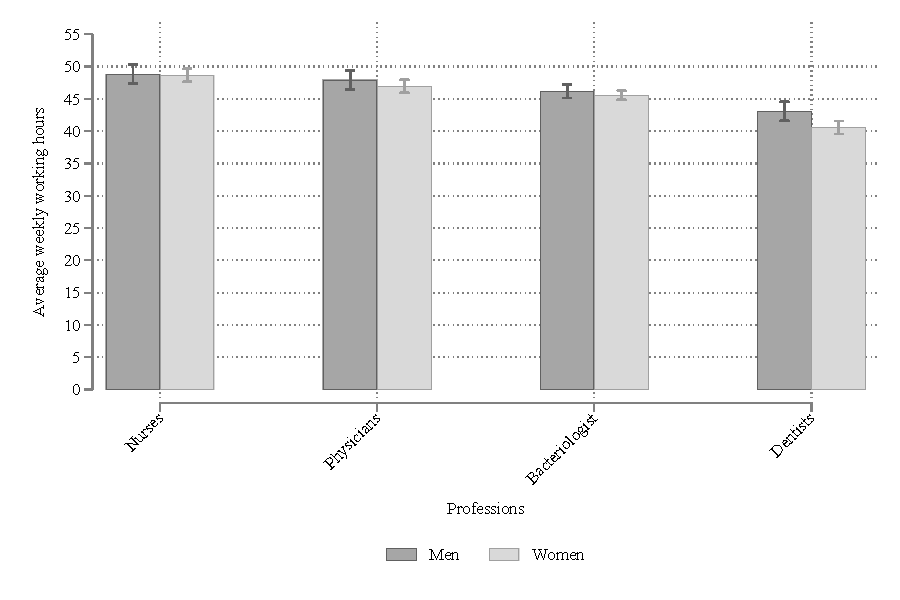
\includegraphics[width=\textwidth]{Figures/hours_gender.pdf}
\fnote{\textit{Notes:} Each bar shows the average weekly working hours of the four professions, using data from the GEIH (2021 to 2023). Confidence intervals are at the 95\% level.}
\end{figure}

\begin{figure}[H]
\caption{Monthly days worked (gender gap)}\label{fig:days_gap}
\centering 
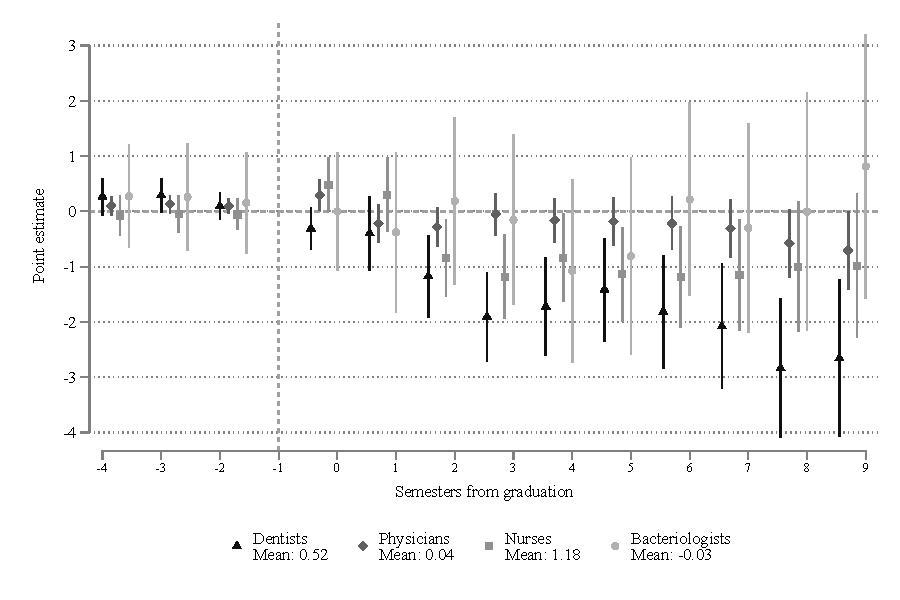
\includegraphics[width=\textwidth]{Figures/Callaway SantAnna/ES_sal_dias_cot_0_gap.pdf}
\fnote{\textit{Notes:} Each point and confidence interval comes from a difference-in-means Welch t-test from the \citet{callaway2021difference} estimations. The confidence intervals are at the 95\% level. The gap at the baseline period (-1) for each profession is reported in the legend. Positive values indicate a gap in favor of men.}
\end{figure}

\begin{figure}[H]
\centering
\caption{Real monthly wages by gender}
\begin{subfigure}{.5\textwidth}
  \centering
  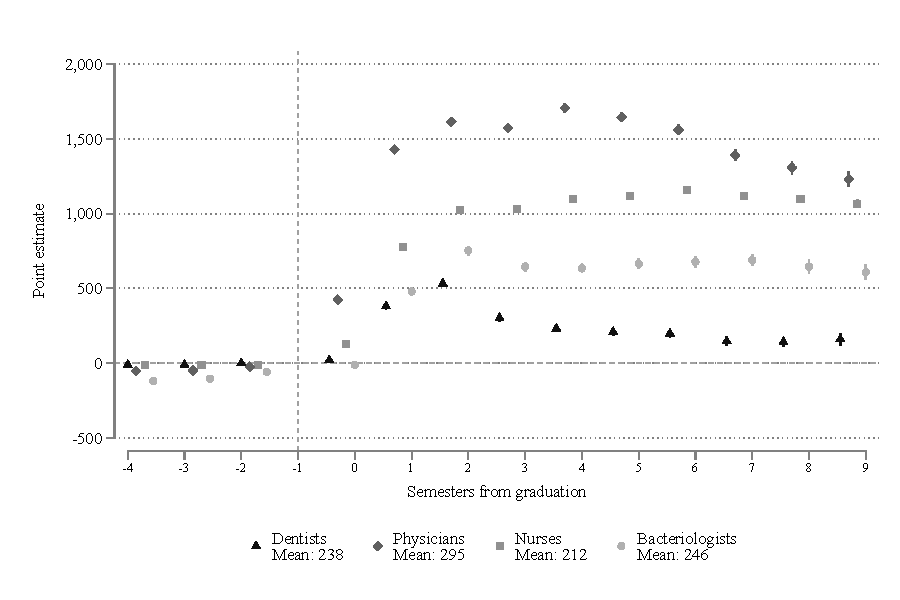
\includegraphics[width=\linewidth]{Figures/Callaway SantAnna/ES_pila_salario_r_0_female.pdf}
  \caption{Females}
  \label{fig:wage_female}
\end{subfigure}%
\begin{subfigure}{.5\textwidth}
  \centering
  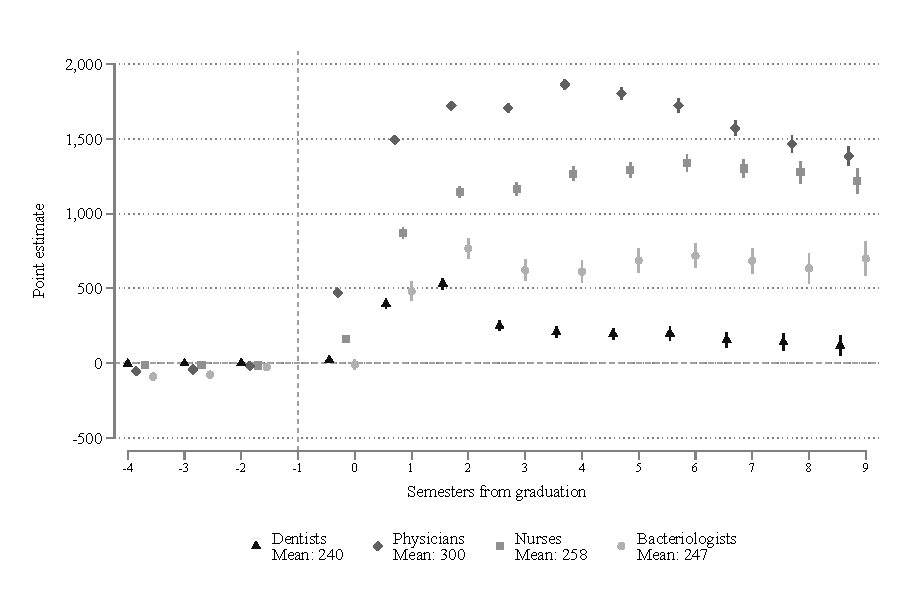
\includegraphics[width=\linewidth]{Figures/Callaway SantAnna/ES_pila_salario_r_0_male.pdf}
  \caption{Males}
  \label{fig:wage_male}
\end{subfigure}
\label{fig:wage_gender}
\fnote{\textit{Notes:} Each point represents a coefficient from the \citet{callaway2021difference} estimation. Wages are in real Colombian Pesos (base 2018). The lines across the coefficients are confidence intervals at the 95\% level. Standard errors are clustered at the individual level. The outcome's mean at the baseline period (-1) for each profession is reported in the legend.}
\end{figure}

\begin{figure}[H]
\caption{Real monthly wage without ever-pregnant women (gender gap)}\label{fig:wage_np_gap}
\centering 
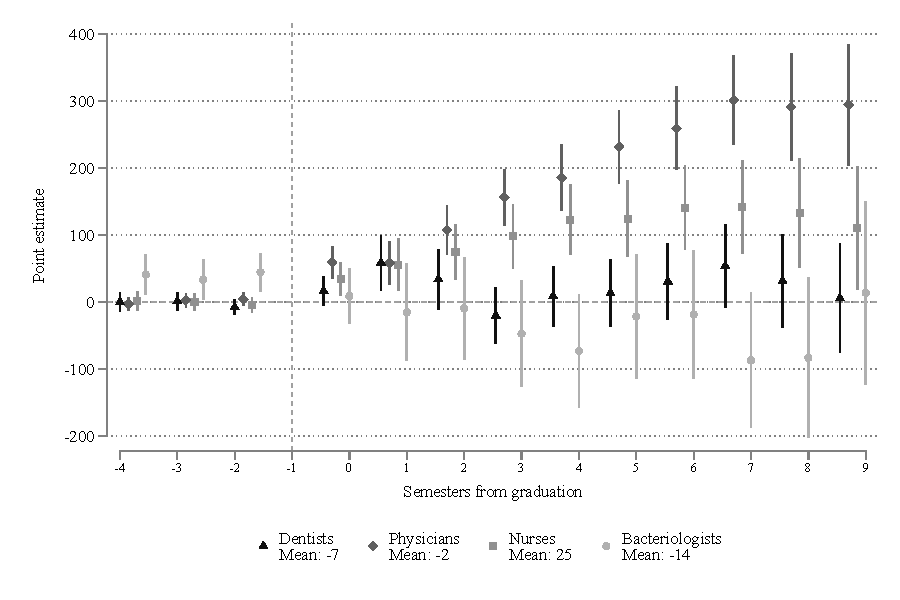
\includegraphics[width=\textwidth]{Figures/Callaway SantAnna/ES_pila_salario_r_0_np_gap.pdf}
\fnote{\textit{Notes:} Each point represents a coefficient from the \citet{callaway2021difference} estimation. The lines across the coefficients are confidence intervals at the 95\% level. Standard errors are clustered at the individual level. The outcome's mean at the baseline period (-1) for each profession is reported in the legend.}
\end{figure}

\begin{figure}[H]
\caption{Probability of being pregnant}\label{fig:pregnancy}
\centering 
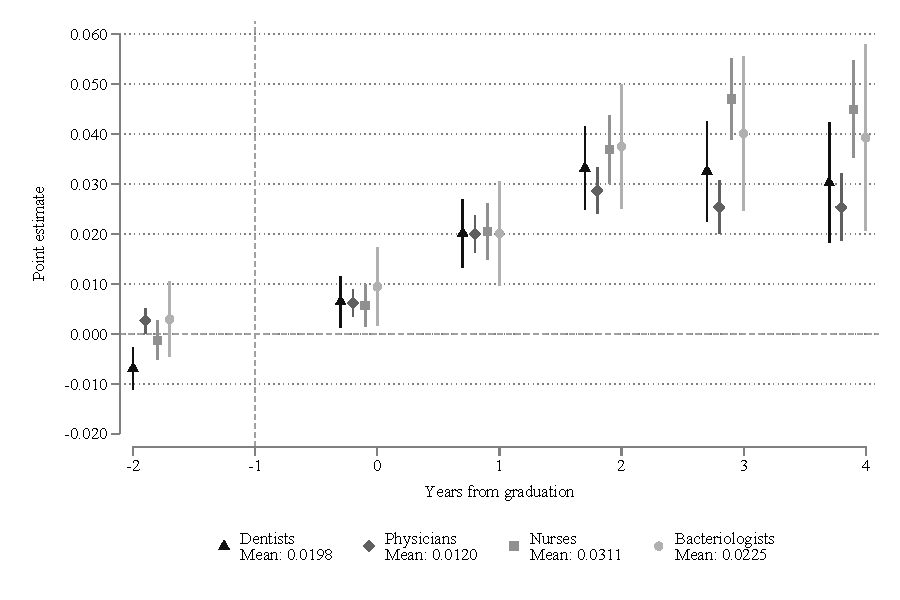
\includegraphics[width=\textwidth]{Figures/Callaway SantAnna/ES_pregnancy_female.pdf}
\fnote{\textit{Notes:} Each point represents a coefficient from the \citet{callaway2021difference} estimation. The lines across the coefficients are confidence intervals at the 95\% level. Standard errors are clustered at the individual level. The outcome's mean at the baseline period (-1) for each profession is reported in the legend.}
\end{figure}

\begin{figure}[H]
\caption{Probability of having multiple jobs (gender gap)}\label{fig:numberjobs_gap}
\centering 
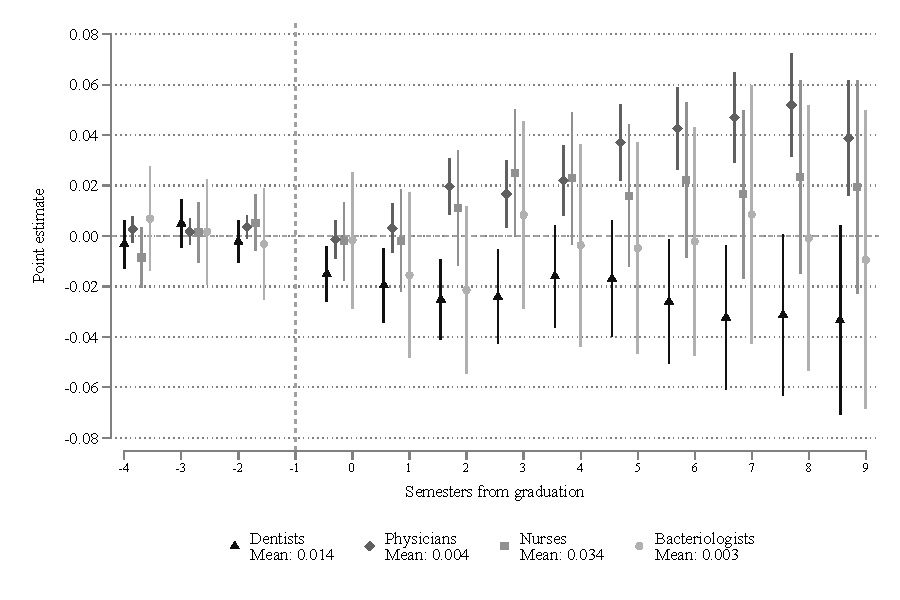
\includegraphics[width=\textwidth]{Figures/Callaway SantAnna/ES_p_cotizaciones_0_gap.pdf}
\fnote{\textit{Notes:} Each point and confidence interval comes from a difference-in-means Welch t-test from the \citet{callaway2021difference} estimations. The confidence intervals are at the 95\% level. The gap at the baseline period (-1) for each profession is reported in the legend. Positive values indicate a gap in favor of men.}
\end{figure}

\begin{figure}[H]
\caption{Alternative gender wage gap}\label{fig:wage_max_gap}
\centering 
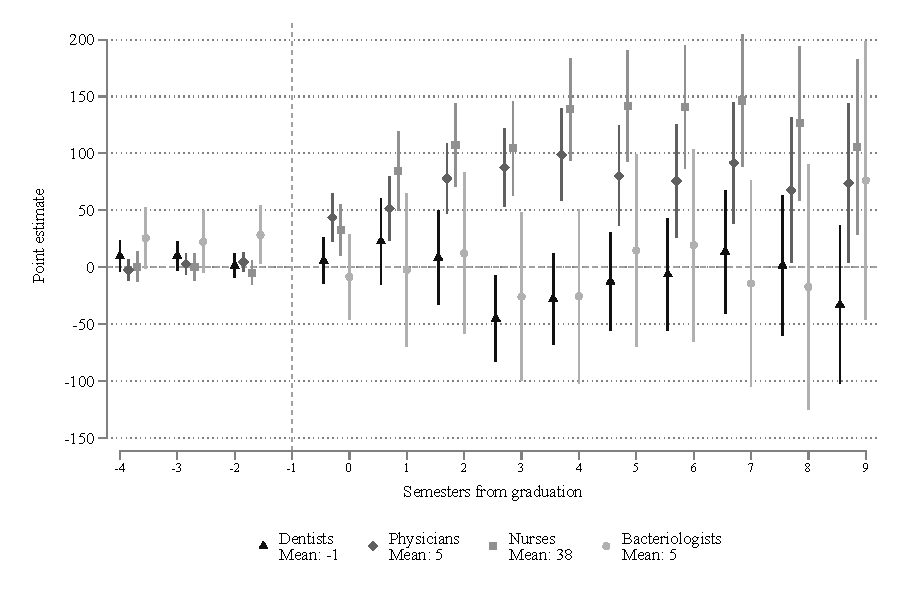
\includegraphics[width=\textwidth]{Figures/Callaway SantAnna/ES_pila_salario_r_max_0_gap.pdf}
\fnote{\textit{Notes:} Each point and confidence interval comes from a difference-in-means Welch t-test from the \citet{callaway2021difference} estimations. Wages are in real Colombian Pesos (base 2018). The confidence intervals are at the 95\% level. The gap at the baseline period (-1) for each profession is reported in the legend. Positive values indicate a gap in favor of men. In this figure, the maximum wage across jobs per person is used, instead of the sum.}
\end{figure}

\begin{figure}[H]
\centering
\caption{Probability of enrollment in a health-related postgraduate program by gender}
\begin{subfigure}{.5\textwidth}
  \centering
  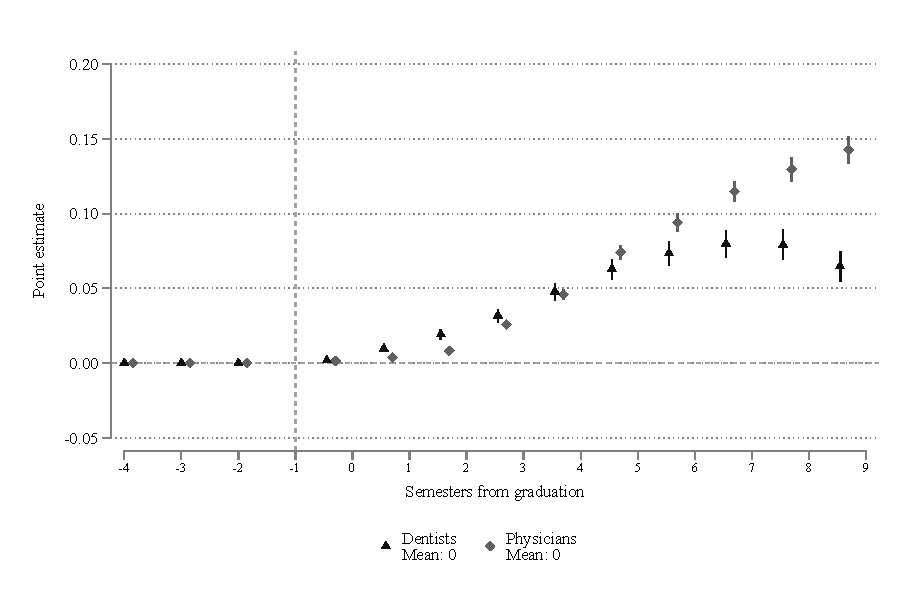
\includegraphics[width=\linewidth]{Figures/Callaway SantAnna/ES_posgrado_salud_female.pdf}
  \caption{Females}
  \label{fig:postgrad_female}
\end{subfigure}%
\begin{subfigure}{.5\textwidth}
  \centering
  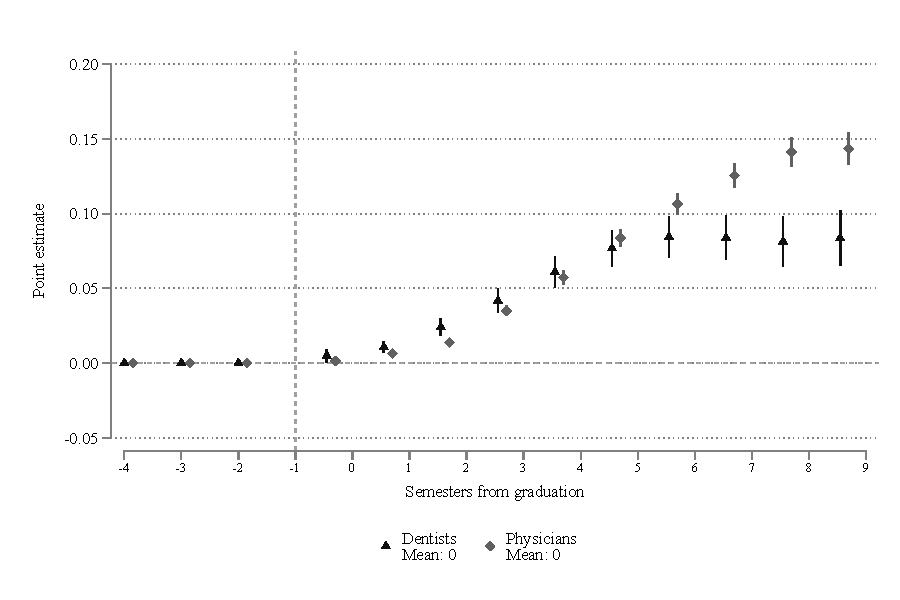
\includegraphics[width=\linewidth]{Figures/Callaway SantAnna/ES_posgrado_salud_male.pdf}
  \caption{Males}
  \label{fig:postgrad_male}
\end{subfigure}
\label{fig:postgrad_gender}
\fnote{\textit{Notes:} Each point represents a coefficient from the \citet{callaway2021difference} estimation. The lines across the coefficients are confidence intervals at the 95\% level. Standard errors are clustered at the individual level. The outcome's mean at the baseline period (-1) for each profession is reported in the legend.}
\end{figure}

\begin{figure}[H]
\centering
\caption{Real monthly wages conditional on postgraduate enrollment (gender gap)}
\begin{subfigure}{.5\textwidth}
  \centering
  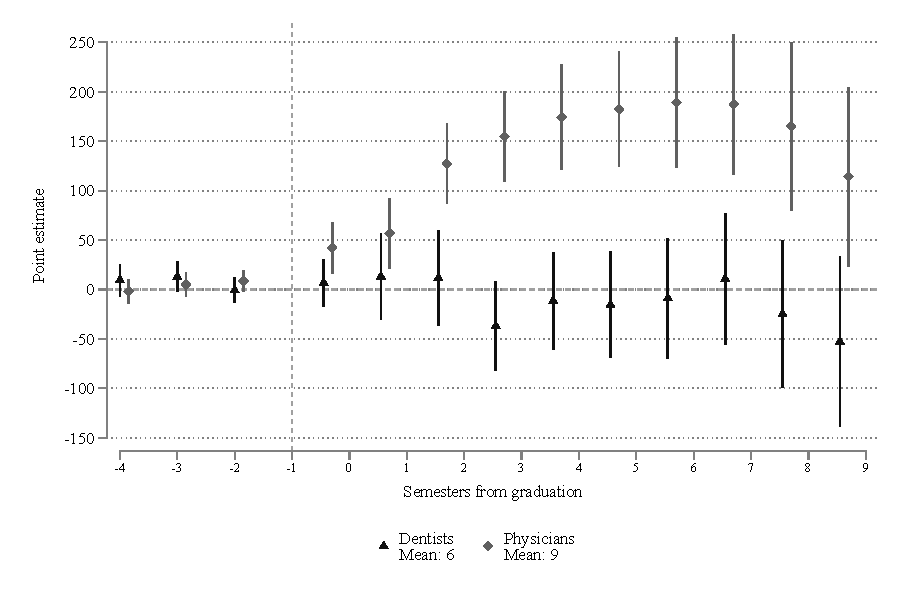
\includegraphics[width=\linewidth]{Figures/Callaway SantAnna/ES_pila_salario_r_0_npos_gap.pdf}
  \caption{Never-enrolled}
  \label{fig:wage_gap_posg}
\end{subfigure}%
\begin{subfigure}{.5\textwidth}
  \centering
  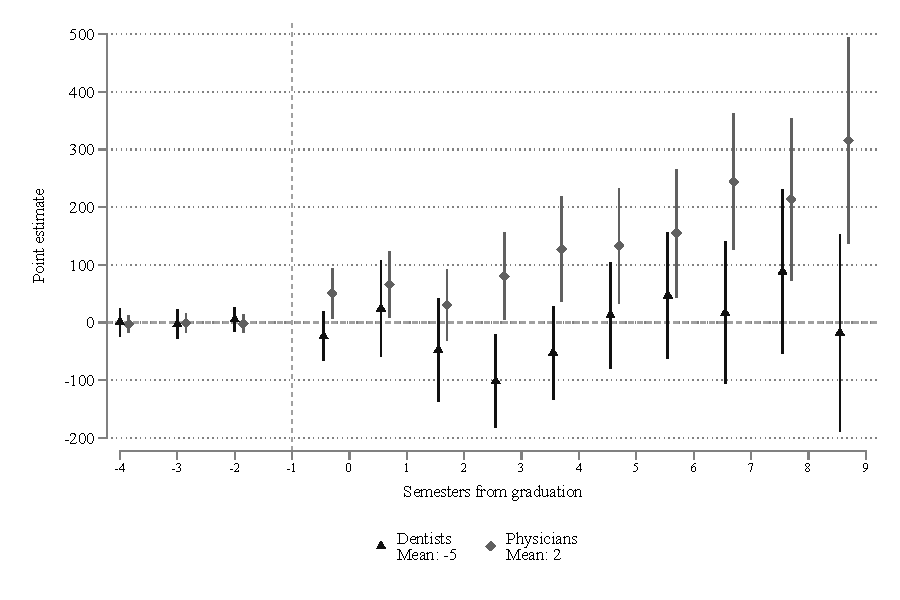
\includegraphics[width=\linewidth]{Figures/Callaway SantAnna/ES_pila_salario_r_0_posg_gap.pdf}
  \caption{Eventually-enrolled}
  \label{fig:wage_gap_npos}
\end{subfigure}
\label{fig:wage_gap_pos}
\fnote{\textit{Notes:} Each point and confidence interval comes from a difference-in-means Welch t-test from the \citet{callaway2021difference} estimations. Wages are in real Colombian Pesos (base 2018). The confidence intervals are at the 95\% level. The gap at the baseline period (-1) for each profession is reported in the legend. Positive values indicate a gap in favor of men. In this figure, the maximum wage across jobs per person is used, instead of the sum.}
\end{figure}

\section{Health trajectories appendix}

\begin{figure}[H]
\caption{Probability of going to the ER (gender gap)}\label{fig:er_gap}
\centering 
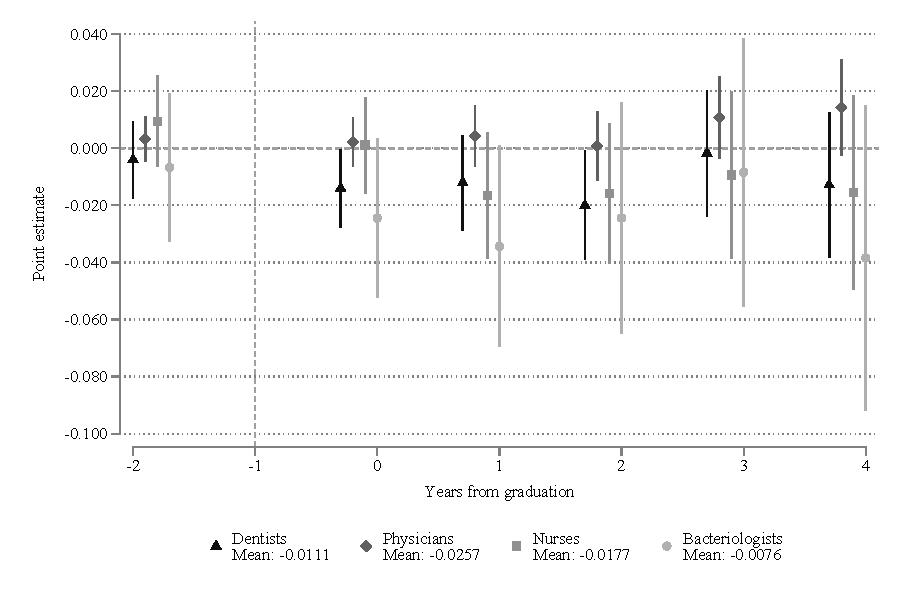
\includegraphics[width=\textwidth]{Figures/Callaway SantAnna/ES_urg_gap.pdf}
\fnote{\textit{Notes:} Each point and confidence interval comes from a difference-in-means Welch t-test from the \citet{callaway2021difference} estimations. The confidence intervals are at the 95\% level. The gap at the baseline period (-1) for each profession is reported in the legend. Positive values indicate a gap in favor of men.}
\end{figure}

\begin{figure}[H]
\caption{Probability of going to the ER from non-pregnancy causes for women}\label{fig:er_np_female}
\centering 
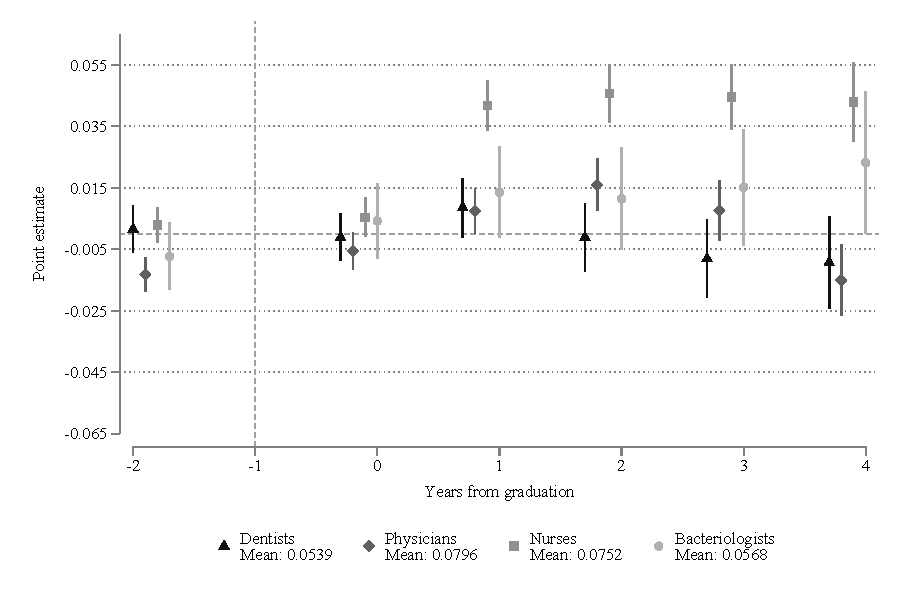
\includegraphics[width=\textwidth]{Figures/Callaway SantAnna/ES_urg_np_female.pdf}
\fnote{\textit{Notes:} Each point represents a coefficient from the \citet{callaway2021difference} estimation. The lines across the coefficients are confidence intervals at the 95\% level. Standard errors are clustered at the individual level. The outcome's mean at the baseline period (-1) for each profession is reported in the legend.}
\end{figure}

\begin{figure}[H]
\caption{Probability of hospitalization (gender gap)}\label{fig:hosp_gap}
\centering 
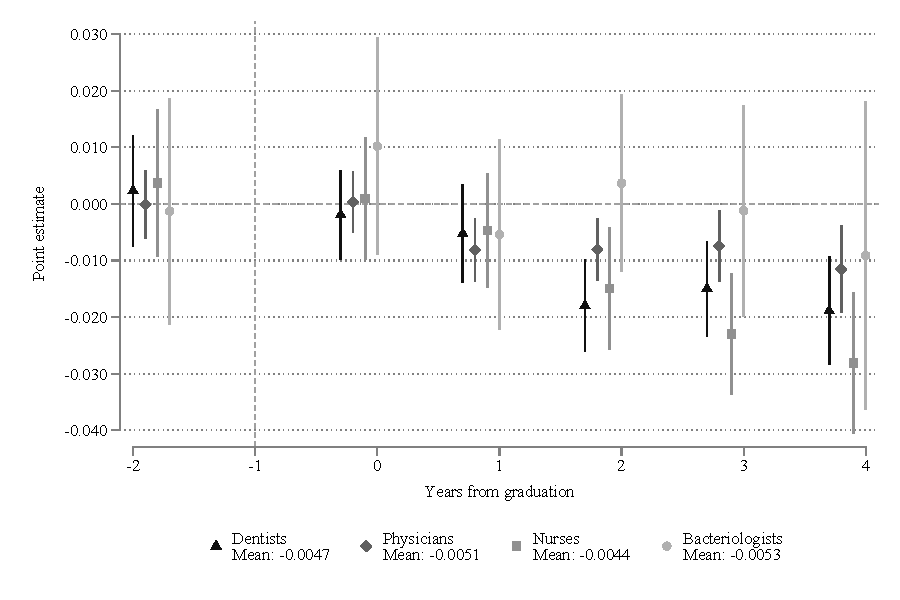
\includegraphics[width=\textwidth]{Figures/Callaway SantAnna/ES_hosp_gap.pdf}
\fnote{\textit{Notes:} Each point and confidence interval comes from a difference-in-means Welch t-test from the \citet{callaway2021difference} estimations. The confidence intervals are at the 95\% level. The gap at the baseline period (-1) for each profession is reported in the legend. Positive values indicate a gap in favor of men.}
\end{figure}

\begin{figure}[H]
\centering
\caption{Probability of hospitalization from non-pregnancy causes for women and gender gap}
\begin{subfigure}{.5\textwidth}
  \centering
  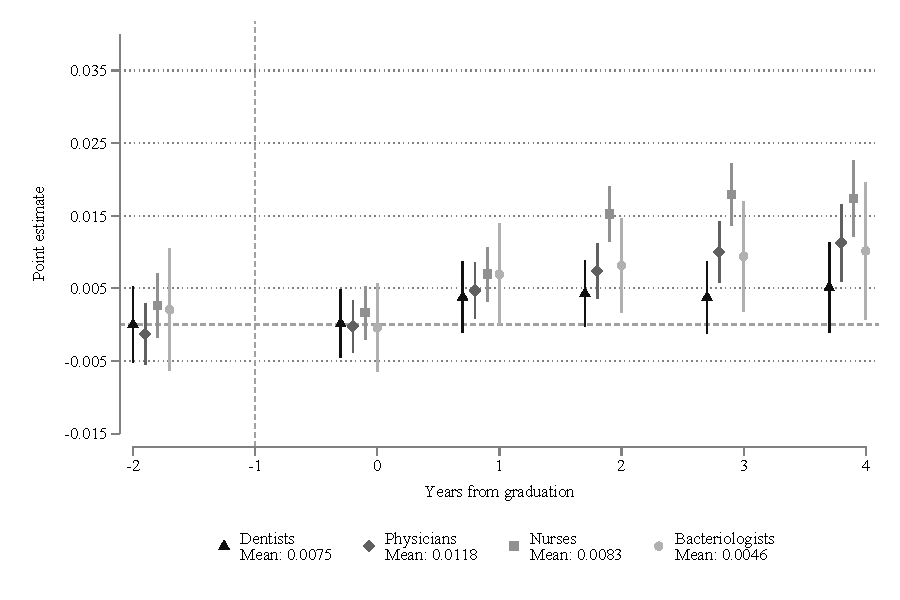
\includegraphics[width=\linewidth]{Figures/Callaway SantAnna/ES_hosp_np_female.pdf}
  \caption{Probability}
  \label{fig:hosp_np_female}
\end{subfigure}%
\begin{subfigure}{.5\textwidth}
  \centering
  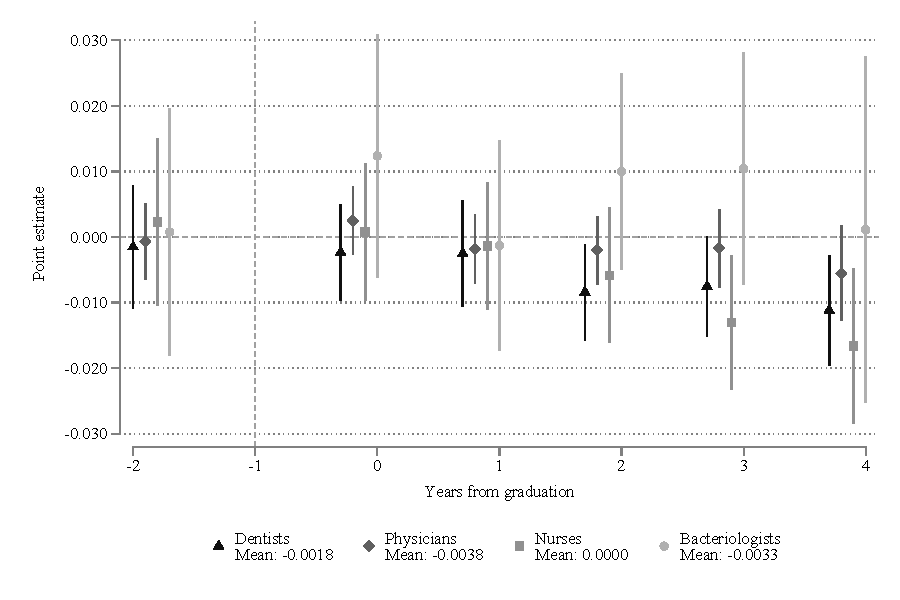
\includegraphics[width=\linewidth]{Figures/Callaway SantAnna/ES_hosp_np_gap.pdf}
  \caption{Gap}
  \label{fig:hosp__npgap}
\end{subfigure}
\label{fig:hosp_np_gap}
\fnote{\textit{Notes:} In the left figure, each point represents a coefficient from the \citet{callaway2021difference} estimation. The lines across the coefficients are confidence intervals at the 95\% level. Standard errors are clustered at the individual level. The outcome's mean at the baseline period (-1) for each profession is reported in the legend. In the figure to the right, each point and confidence interval comes from a difference-in-means Welch t-test from the \citet{callaway2021difference} estimations. The confidence intervals are at the 95\% level. The gap at the baseline period (-1) for each profession is reported in the legend. Positive values indicate a gap in favor of men.}
\end{figure}

\begin{figure}[H]
\caption{Probability of having a mental condition (gender gap)}\label{fig:mental_forever_gap}
\centering 
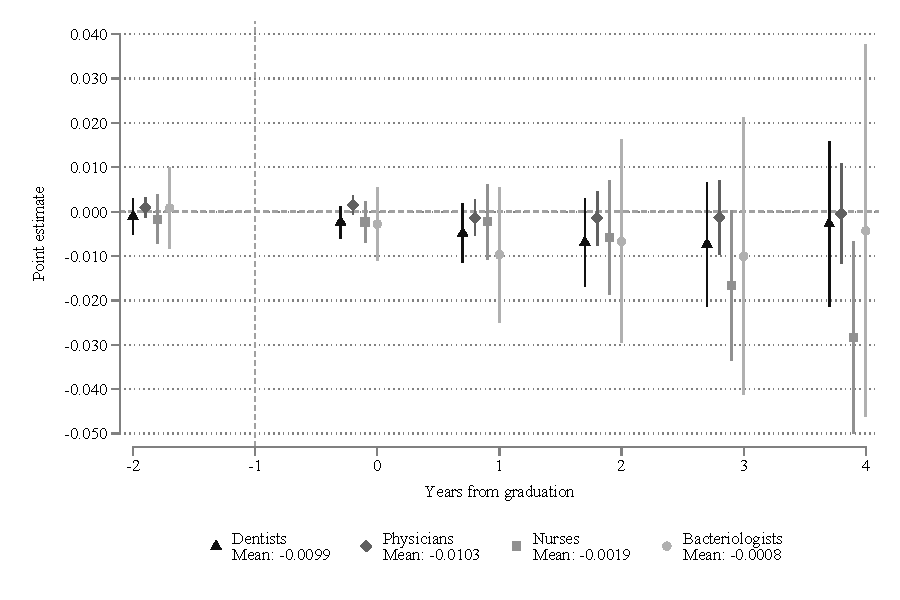
\includegraphics[width=\textwidth]{Figures/Callaway SantAnna/ES_service_mental_forever_gap.pdf}
\fnote{\textit{Notes:} Each point and confidence interval comes from a difference-in-means Welch t-test from the \citet{callaway2021difference} estimations. The confidence intervals are at the 95\% level. The gap at the baseline period (-1) for each profession is reported in the legend. Positive values indicate a gap in favor of men.}
\end{figure}

\end{document}